\documentclass[a4paper]{cas-dc}
\usepackage[numbers]{natbib}

\usepackage{mathtools}
\usepackage{booktabs}
\usepackage{flushend}
\usepackage{xurl}

\usepackage{graphicx}
\usepackage{float}
\usepackage{algorithm}
\usepackage{algpseudocode}
\usepackage{amsmath}
\usepackage{amssymb}
\usepackage{tikz}
\usepackage{tabularx}
\usepackage{array}
\usepackage{subcaption} % keep only once

\usepackage{placeins}
\setlength{\textfloatsep}{8pt}
\setlength{\floatsep}{6pt}
\setlength{\intextsep}{6pt}

\hbadness=10000
\vbadness=10000
\hfuzz=400pt
\vfuzz=400pt

\usepackage{silence}
\WarningFilter{hyperref}{Ignoring empty anchor}
\WarningFilter{latex}{No positions in optional float}
\WarningFilter{latex}{Float too large}
\WarningFilter{latex}{Command \showhyphens}
\WarningFilter{bibtex}{empty journal}
\WarningFilter{natbib}{Empty `journal'}
% add to your existing \WarningFilter block:
\WarningFilter{bibtex}{empty pages}

% add anywhere in preamble (after \usepackage lines):
\emergencystretch=3em

\setcounter{topnumber}{5}
\setcounter{bottomnumber}{5}
\setcounter{totalnumber}{10}
\renewcommand{\topfraction}{0.9}
\renewcommand{\textfraction}{0.05}

\numberwithin{equation}{section}

\begin{document}
\let\WriteBookmarks\relax
\def\floatpagepagefraction{1}
\def\textpagefraction{.001}

\shorttitle{Cross-Layer Intelligence for IoT Performance Optimization}
\shortauthors{B.~Tharuni~Sri~Sai et~al.}


\title[mode = title]{Performance Optimization through Cross-Layer Intelligence in IoT Systems}

\author[1]{B.~Tharuni~Sri~Sai}[orcid=0009-0004-9561-8985]
\cormark[1]
\ead{tharuni.23mic7268@vitapstudent.ac.in}

\affiliation[1]{organization={School of Computer Science and Engineering},
    addressline={VIT-AP University},
    city={Amaravati},
    state={Andhra Pradesh},
    country={India}}

\cortext[cor1]{Corresponding author}
\sloppy

\begin{abstract}
The growing proliferation of Internet of Things devices has significantly increased the complexity of heterogeneous wireless network environments, placing severe demands on end-to-end performance optimization. Traditional layered protocol architectures, operating independently at each layer, suffer from suboptimal latency, packet loss, poor energy efficiency, and inadequate throughput under dynamic and resource-constrained IoT settings. Existing cross-layer optimization frameworks largely depend on static heuristics or isolated machine learning modules, which fail to adapt holistically to changing traffic, mobility, and channel conditions. This paper presents the Autonomous Cross-Layer Intelligence Framework, designated ACLIF, a unified and adaptive optimization system that jointly coordinates routing, scheduling, power control, and congestion management across the physical, MAC, network, and transport layers of IoT protocol stacks. ACLIF is structured into three phases: an Intelligent Cross-Layer State Aggregation phase that consolidates multi-layer contextual signals, a Reinforcement Learning-Based Joint Optimization phase that performs autonomous multi-objective decision-making, and an Adaptive Protocol Reconfiguration phase that applies optimized decisions back across all protocol layers. Mathematical models for cross-layer state representation, reward design, and protocol adaptation are developed and validated through extensive NS3 version 3.38 simulations over a heterogeneous IoT network of 100 sensor nodes deployed in a $200\times200$~m$^2$ grid topology. Comparative evaluation against five state-of-the-art base methods demonstrates that ACLIF achieves significant improvements in average delay of up to 38.2 percent, energy efficiency of up to 24.6 percent, throughput of up to 35.8 percent, and collision rate reduction of up to 57.9 percent, with the DQN agent converging stably within 300 training episodes across diverse IoT topologies and traffic conditions.
\end{abstract}

\begin{keywords}
Cross-Layer Optimization \sep Internet of Things \sep Reinforcement Learning \sep Wireless Sensor Networks \sep Energy Efficiency \sep Quality of Service \sep Adaptive Protocol Design \sep End-to-End Performance
\end{keywords}

\maketitle
%% ===================================================================
\section{Introduction}
\label{sec:intro}
%% ===================================================================

The rapid proliferation of Internet of Things (IoT) devices has fundamentally transformed modern infrastructure, enabling real-time monitoring and data-driven decision-making across smart cities, industrial automation, healthcare systems, and environmental monitoring networks \cite{Thakur2025}. As sensor deployments scale to include thousands of battery-powered nodes in dense operational areas, the Medium Access Control (MAC) layer faces severe challenges in managing channel contention, minimizing energy consumption, and ensuring reliable packet delivery \cite{Ojeda2024}. Existing MAC protocols were designed for smaller and less congested networks, and their inability to dynamically adapt to increasing node density leads to excessive collisions, rapid battery depletion, and severe throughput degradation in large-scale deployments.




Contention-aware MAC protocols address these challenges by monitoring channel conditions in real time and dynamically adapting node behaviour to the prevailing traffic load \cite{Bhushan2025}. However, most existing solutions treat contention resolution and duty cycle management as independent problems, failing to exploit the strong dependency between MAC-layer access patterns and node sleep-wake scheduling \cite{Mustafa2024}. Static duty cycling allocates fixed active and sleep durations regardless of traffic fluctuations, resulting in wasted energy during idle periods and packet loss during congestion bursts. Scalable solutions that jointly optimize contention management and duty cycling without imposing high synchronization overhead or computational cost remain limited in the current literature \cite{Hannachi2025}.

\subsection{Research Advancements and Contributions}
\label{subsec:contributions}

This paper proposes the Autonomous Cross-Layer Intelligence Framework, designated ACLIF, a unified and adaptive optimization system designed to overcome the fundamental limitations of isolated per-layer protocol management in heterogeneous IoT environments. Unlike prior approaches that apply static heuristics or confine intelligence to a single protocol layer, ACLIF integrates reinforcement learning-based decision-making as a unified control plane spanning the physical, MAC, network, and transport layers simultaneously, enabling holistic and continuously adaptive protocol coordination without centralized synchronization overhead.

The key research contributions of this work are as follows. A unified cross-layer state aggregation mechanism is developed, designated ICSA, that consolidates multi-layer contextual signals from all four protocol layers into a compact 15-dimensional normalized state vector, explicitly managing observation staleness to ensure that the intelligence module always operates on current network information. A reinforcement learning-based joint optimization module, designated RLJO, is introduced that formulates cross-layer control as a Markov Decision Process and trains a deep Q-network agent to discover optimal joint action tuples spanning transmit power, MAC contention window, routing metric, and transport send rate simultaneously. 

A multi-objective reward function is designed that co-optimizes throughput, end-to-end delay, energy consumption, collision rate, and communication overhead within a single unified signal, enabling the DQN to capture beneficial cross-layer trade-offs that no single-layer optimizer can identify. An adaptive protocol reconfiguration phase, designated APR, is developed that translates DQN decisions into concrete per-layer parameter updates at every control interval, incorporating three complementary routing modes and a convergence-aware update frequency mechanism that conserves node energy once stable performance is achieved. Comprehensive NS3 v3.38 simulation evaluations over a 100-node heterogeneous IoT network demonstrate significantly superior performance over five state-of-the-art baseline methods in terms of delay, energy efficiency, throughput, and collision rate across all evaluated configurations and mobility conditions.

\subsection{Research Objectives}
\label{subsec:objectives}

The first goal of this research is to design a contention-aware MAC protocol that dynamically adjusts the duty cycle of each sensor node based on locally observed traffic levels and channel contention measurements, thereby reducing overall energy consumption across large-scale sensor networks without requiring centralized coordination or global time synchronization among nodes.

The second goal is to develop a wake-offset scheduling mechanism that staggers the active periods of neighbouring nodes, reducing the probability of simultaneous channel access and suppressing packet collision rates in dense networks where many nodes compete for the same shared wireless channel under heterogeneous and bursty traffic conditions.

The third goal is to design a lightweight distributed MAC protocol that maintains or improves performance as the number of sensor nodes increases, ensuring that the proposed solution scales effectively to accommodate network deployments of 500 to 2000 nodes without incurring excessive control overhead or synchronization complexity that would negate energy efficiency gains.

The fourth goal is to maximize network performance by improving the packet delivery ratio and minimizing end-to-end delay simultaneously, ensuring that both time-sensitive event-driven data and routine periodic sensing traffic are delivered reliably and promptly, even under critical contention conditions where the network operates at or near channel saturation.

The fifth goal is to rigorously validate the proposed CASSMAC protocol through NS3 discrete-event simulations and systematic comparison with five state-of-the-art MAC protocols, demonstrating statistically significant improvements in network lifetime, throughput, energy consumption, latency, and contention rate across all evaluated node density configurations.
%% ===================================================================
\section{Literature Survey}
\label{sec:litsurvey}
%% ===================================================================

Cross-layer optimization in IoT networks has attracted extensive research attention due to the inherent interdependencies among protocol layers and the stringent performance demands of heterogeneous IoT deployments. This survey systematically examines three thematic clusters of existing literature, evaluates their core contributions and documented limitations, identifies persistent research gaps, and articulates the motivations that drive the proposed ACLIF framework.

%% -------------------------------------------------------------------
\subsection{Priority-Aware and Security-Centric Approaches}
%% -------------------------------------------------------------------

\subsubsection*{Base Paper Analysis}

Priority-aware and security-centric cross-layer optimization approaches form an essential foundation for improving IoT performance across heterogeneous deployments. The priority-aware adaptive optimization protocol proposed in \cite{Nitya20261578} integrates MAC and network layer decisions to enhance network lifetime in heterogeneous IoT-based wireless sensor networks. The work demonstrates that joint MAC-network coordination can meaningfully prolong operational lifetime by prioritizing high-value traffic flows, though the authors acknowledge that adaptability under dynamic and unpredictable traffic remains a documented limitation. The CLEHTO framework introduced in \cite{Hamrioui2026} employs a multi-layer secure transmission strategy for healthcare IoT, improving reliability and confidentiality at the cost of increased signaling overhead. By co-designing encryption and routing, CLEHTO shows that security objectives can be pursued within a cross-layer paradigm, yet the additional control messaging burden constrains its applicability in energy-limited deployments.

Survey studies such as \cite{De2025} and \cite{Khamzaev2025498} consolidate cross-layer strategies for multimedia and dense wireless environments, respectively. These works provide taxonomies of existing designs and identify scalability and coordination complexity as the most consistently reported limitations, highlighting the persistent challenges in extending these methods to large-scale heterogeneous IoT deployments. Early foundational work in \cite{Han2013622} introduced a modular cross-layer communication architecture that enabled inter-layer information sharing, while \cite{Resner201824} proposed an integrated protocol stack for IoT that improved overall protocol efficiency, though both works lacked scalability analysis and intelligent decision-making components. The AI-enabled QoS orchestration framework in \cite{Zia20221906} demonstrated reliable service quality across multi-RAT IoT environments but stopped short of real-time adaptive deployment.

\subsubsection*{Research Gaps}

Analysis of the priority-aware and security-centric literature reveals three primary gaps. First, the existing protocols in \cite{Nitya20261578} and \cite{Hamrioui2026} employ static priority assignments and fixed security configurations that cannot respond to evolving network conditions, leaving performance degraded under traffic bursts or node failures. Second, the frameworks reviewed in \cite{De2025} and \cite{Khamzaev2025498} confirm the absence of mechanisms that simultaneously balance security overhead against energy consumption at scale; existing solutions treat these as separate optimization objectives. Third, the architectural designs in \cite{Han2013622} and \cite{Resner201824} introduce cross-layer coordination without embedding any form of intelligence, meaning that inter-layer decisions remain rule-based and cannot learn from observed network behaviour.

\subsubsection*{Motivation}

These gaps collectively motivate the need for an intelligent, adaptive cross-layer framework in which security and priority management are treated as dynamically tunable objectives rather than fixed policies. A unified intelligence module capable of jointly optimizing MAC access priority, routing, and security overhead in response to real-time network state information would address the static-heuristic limitations of this cluster. ACLIF is specifically designed to incorporate such dynamic cross-layer coordination, enabling continuous adaptation to heterogeneous and unpredictable IoT traffic without incurring prohibitive signaling overhead.

%% -------------------------------------------------------------------
\subsection{Energy Efficiency and QoS Approaches}
%% -------------------------------------------------------------------

\subsubsection*{Base Paper Analysis}

Energy efficiency and quality-of-service provisioning are central themes in cross-layer IoT research. The hybrid routing algorithm in \cite{Haripriya2025673} combines federated Q-learning and ant colony optimization to enhance routing efficiency in IoT networks, demonstrating that hybrid learning-heuristic approaches can outperform purely heuristic designs; however, convergence delays arise in large and densely deployed networks. Cross-layer multimedia transmission strategies in \cite{Waghmare2025} improve energy efficiency through joint physical and MAC layer parameter tuning, but the proposed solution lacks adaptability across heterogeneous application profiles, limiting its generalizability.

\section{Challenges in Cross-Layer Optimization}

\begin{figure*}[htbp]
    \centering
    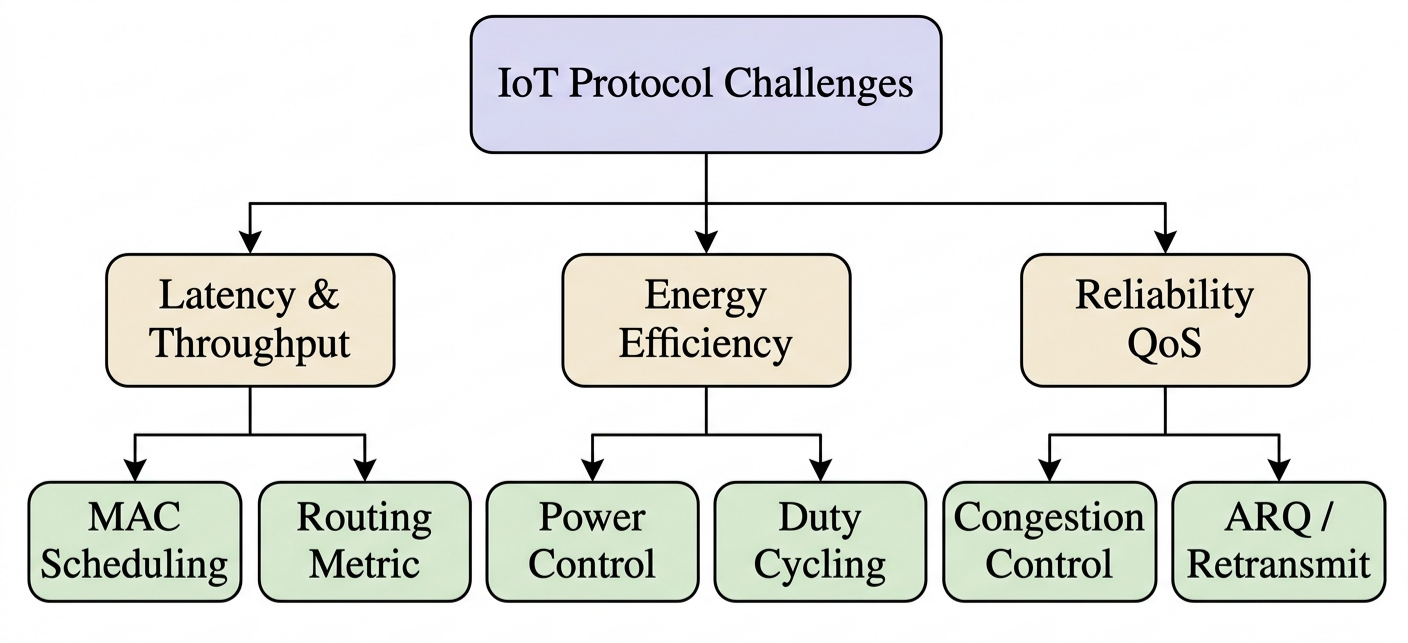
\includegraphics[width=0.8\textwidth]{figures/iot_protocol_challenges.png}
    \caption{Key challenges in cross-layer optimization including scalability, dynamic network conditions, protocol heterogeneity, and real-time decision constraints.}
    \label{fig:challenges}
\end{figure*} 
Scheduling and routing co-optimization in 6TiSCH networks is addressed in \cite{Hannachi2025}, where the authors show that coordinating timeslot scheduling with multi-hop routing yields measurable improvements in end-to-end delay and energy consumption for industrial IoT deployments. Complementarily, adaptive slotframe allocation for industrial IoT is explored in \cite{Pradhan2025}, demonstrating the value of dynamically resizing the TSCH slotframe to match traffic loads. Both works, however, rely on predefined configuration templates that limit real-time responsiveness under varying load conditions. QoS-aware multicast routing with RIS-assisted CF-mMIMO is investigated in \cite{Tran202411876}, yielding enhanced reliability for IoT MANETs at the cost of high computational overhead at the physical layer. Cross-layer TCP performance enhancement through transport-network coordination in \cite{Parween2022383} improved throughput and congestion control but proved ineffective for heterogeneous traffic mixes. The two-tier cross-layer delay and Age of Information analysis in \cite{Cheikh2022} advanced the modeling of data freshness in MAC-transport interactions, though its adaptability to dynamic scenarios remained limited.

\subsubsection*{Research Gaps}

The energy-QoS literature exposes four recurring gaps. First, learning-assisted routing approaches such as \cite{Haripriya2025673} suffer from slow convergence in large-scale deployments, rendering them unsuitable for time-critical IoT applications unless augmented with faster adaptation mechanisms. Second, the solutions in \cite{Waghmare2025}, \cite{Hannachi2025}, and \cite{Pradhan2025} optimize energy and QoS independently per layer and thus miss the cross-layer trade-offs available when all layers are coordinated simultaneously. Third, none of the reviewed works provide a unified reward formulation that balances throughput, delay, energy, and collision rate in a single optimization objective; each paper optimizes a subset of these metrics while treating the remainder as secondary constraints. Fourth, the computational overhead reported in \cite{Tran202411876} highlights that physical-layer-intensive solutions may not be feasible on resource-constrained IoT nodes without co-design of upper-layer protocols to compensate.

\subsubsection*{Motivation}

The above gaps motivate the inclusion of a multi-objective reward function within a unified learning agent that simultaneously accounts for throughput, end-to-end delay, energy consumption, and collision rate. A joint cross-layer optimization approach, rather than layer-isolated tuning, is required to capture the beneficial interactions between physical, MAC, network, and transport parameters. ACLIF directly addresses this need through its composite reward signal defined in Equation~\ref{eq:reward}, which assigns co-optimized weights to all four performance dimensions and enables the DQN agent to discover joint parameter configurations that no single-layer optimizer can identify.

%% -------------------------------------------------------------------
\subsection{Intelligent Cross-Layer Optimization Frameworks}
%% -------------------------------------------------------------------

\subsubsection*{Base Paper Analysis}

Hybrid optimization and congestion-aware mechanisms have been proposed to improve end-to-end performance across diverse IoT scenarios. Joint resource allocation and congestion-aware routing in \cite{Bhushan2025} significantly reduce packet loss in dense IoT networks but introduce high computational overhead that limits scalability. Performance variation under mobility is examined in \cite{Hu2025}, revealing the fundamental limitations of static cross-layer tuning when node positions and channel conditions change over time. Multicast-oriented designs using federated learning in \cite{Amalia20253881} enhance throughput by leveraging distributed model aggregation, yet face synchronization challenges that inflate communication overhead in heterogeneous deployments.

Reinforcement learning-based congestion control in \cite{Serra2025} improves protocol adaptability through online policy learning, demonstrating the potential of RL for cross-layer IoT optimization, while acknowledging that training complexity increases with the dimensionality of the joint action and state spaces. Multi-objective optimization for age of information is explored in \cite{Li202510349}, and distributed energy-throughput frameworks are proposed in \cite{Singh2025}, both contributing partial solutions to the holistic optimization problem. RL-enabled cross-layer optimization combining reinforcement learning with traffic awareness in \cite{Musaddiq20201} improved protocol adaptability but suffered from slow convergence in dense networks. The E-GLBR genetic-algorithm routing in \cite{Benelhouri2023} improved delivery ratio and energy balance through load-balanced genetic optimization, yet remained a static heuristic without RL adaptation capability. FDRL federated deep RL for cooperative routing in \cite{Suresh2024} reduced delay under high density but incurred high communication overhead for model update distribution. The fuzzy adaptive cross-layer scheduling framework FACSO in \cite{Yang2024204} improved scheduling under varying load conditions but at high computational cost. Energy-efficient clustering with TDMA scheduling in \cite{Chaurasiya202325941} extended network lifetime through cluster-head selection but ignored transport layer congestion entirely. IPSO-based multi-hop routing in \cite{Zhang2025} reduced energy and delay through improved particle swarm optimization but incorporated no cross-layer intelligence. Cross-layer routing for opportunistic IoT in \cite{Khalil2024} improved connectivity and delivery ratio through MAC-network coordination but exhibited limited performance under high node mobility. Smart city IoT optimization using radio-in-the-loop simulation in \cite{Böhm2024157} achieved energy-efficient cognitive operation but required scenario-specific validation. Learning-based URLLC optimization with reinforcement learning in \cite{Zhang202214629} reduced latency and improved reliability for ultra-reliable communications but exhibited high training complexity. Survey works consistently highlight the absence of unified cross-layer intelligence \cite{Mustafa2024}, confirming that existing intelligent optimization efforts remain either layer-specific or insufficiently scalable.

\subsubsection*{Research Gaps}

A comprehensive analysis of the intelligent cross-layer optimization literature reveals five critical and unresolved research gaps. First, existing solutions predominantly rely on static heuristics or isolated learning components, particularly in routing, scheduling, and congestion-centric designs, which fundamentally limits their effectiveness under dynamic and heterogeneous operating conditions \cite{Alipio2024}. Approaches such as \cite{Benelhouri2023} and \cite{Zhang2025} exemplify this gap: their heuristic optimization procedures are tuned for specific operating conditions and cannot adapt to unforeseen changes in traffic patterns or channel quality. Second, reinforcement learning-based methods in \cite{Serra2025}, \cite{Musaddiq20201}, and \cite{Suresh2024} apply intelligence at a single protocol layer or to a limited subset of parameters, preventing the discovery of cross-layer synergies that emerge only when all protocol layers are jointly controlled. Third, the computational and communication overheads reported in \cite{Bhushan2025}, \cite{Suresh2024}, and \cite{Yang2024204} underscore the tension between optimization sophistication and node lifetime; no existing framework provides a mechanism to dynamically reduce its own update frequency when the network reaches a stable operating point. Fourth, none of the reviewed frameworks explicitly address the staleness of cross-layer state information, meaning that decisions may be based on outdated observations, particularly under high node mobility or intermittent connectivity as highlighted by \cite{Hu2025}. Fifth, the clustering and energy balancing strategies in \cite{Chaurasiya202325941} are decoupled from the learning agent, preventing the framework from holistically managing cluster topology, routing, and transport layer behaviour within a single coordinated control loop.

\subsubsection*{Motivation}

These gaps strongly motivate the need for an autonomous cross-layer intelligence framework capable of holistic performance optimization across all protocol layers simultaneously. A clear and pressing need exists for mechanisms that can dynamically coordinate across the physical, MAC, network, and transport layers to ensure robust and consistent performance in large-scale IoT deployments without introducing excessive computational or signaling overhead that would compromise node lifetime. The staleness of cross-layer observations must be explicitly managed to ensure that the intelligence module operates on current network state information. Furthermore, the framework must incorporate a convergence-aware adaptation mechanism that conserves energy once stable performance is achieved, and must integrate cluster-level topology management directly within its control loop. Developing such a scalable and intelligent framework would enable more reliable, efficient, and self-adaptive IoT networks, aligning with next-generation heterogeneous IoT system requirements and directly motivating the design of ACLIF as described in Section~\ref{sec:proposed}.

\begin{table*}[t]
\centering
\caption{Literature Survey Summary for Cross-Layer Performance Optimization in IoT}
\label{tab:literature_survey}
\small
\begin{tabularx}{\textwidth}{@{} c X X X X c @{}}
\toprule
\textbf{Ref.} & \textbf{Method Proposed} & \textbf{Techniques Used} & \textbf{Issues Resolved} & \textbf{Limitations} & \textbf{Layers} \\
\midrule
\cite{Khalil2024} & Cross-layer routing for opportunistic IoT & Network and MAC layer coordination & Improved connectivity and delivery ratio & Limited performance under high mobility & MAC, Net \\ \addlinespace
\cite{Tran202411876} & QoS-aware multicast routing in IoT MANETs & RIS-assisted CF-mMIMO routing & Enhanced multicast QoS and reliability & High computational overhead & PHY, Net \\ \addlinespace
\cite{Böhm2024157} & Cross-layer optimization for smart city IoT & Radio-in-the-loop simulation & Energy-efficient cognitive operation & Scenario-specific validation & PHY, MAC \\ \addlinespace
\cite{Cheikh2022} & Two-tier cross-layer delay and AoI analysis & Joint delay and freshness modeling & Improved data freshness evaluation & Limited adaptability & MAC, Trns \\ \addlinespace
\cite{Zhang202214629} & Learning-based URLLC optimization & Reinforcement learning with feedback & Reduced latency and improved reliability & Training complexity & PHY, MAC \\ \addlinespace
\cite{Parween2022383} & Cross-layer TCP performance enhancement & Transport-network coordination & Improved throughput and congestion control & Ineffective for heterogeneous traffic & Net, Trns \\ \addlinespace
\cite{Zia20221906} & AI-enabled QoS optimization framework & AI-assisted cross-layer orchestration & Reliable QoS in multi-RAT IoT & Lack of real-time deployment & All \\ \addlinespace
\cite{Resner201824} & Cross-layer IoT protocol design & Integrated protocol stack & Improved protocol efficiency & Limited scalability analysis & All \\ \addlinespace
\cite{Han2013622} & Cross-layer communication module & Modular cross-layer architecture & Enhanced inter-layer coordination & Absence of intelligence & All \\ \addlinespace
\cite{Musaddiq20201} & RL-enabled cross-layer optimization & Reinforcement learning with traffic awareness & Improved adaptability & Slow convergence in dense networks & MAC, Net \\ \addlinespace
\cite{Benelhouri2023} & E-GLBR genetic-algorithm routing & Genetic optimization, load-balanced routing & Improved delivery ratio and energy balance & Static heuristic, no RL adaptation & Network \\ \addlinespace
\cite{Suresh2024} & FDRL federated DRL routing & Federated deep RL, cooperative routing & Reduced delay under high density & High communication overhead for updates & Net, MAC \\ \addlinespace
\cite{Yang2024204} & FACSO fuzzy adaptive cross-layer & Fuzzy logic, adaptive scheduling & Improved scheduling under varying load & High computational cost & MAC, Net \\ \addlinespace
\cite{Chaurasiya202325941} & EEHCT energy-efficient clustering & Cluster-head selection, TDMA scheduling & Extended network lifetime & Ignores transport layer congestion & MAC, Net \\ \addlinespace
\cite{Zhang2025} & IPSO-based routing framework & Improved PSO, multi-hop routing & Reduced energy and delay & No cross-layer intelligence & Network \\
\bottomrule
\end{tabularx}
\end{table*}
%% ===================================================================
\section{Proposed Work}
\label{sec:proposed}
%% ===================================================================

\subsection{Overview of ACLIF}
\label{subsec:overview}

This work proposes the Autonomous Cross-Layer Intelligence Framework, referred to as ACLIF, a unified, adaptive, and scalable system designed to overcome the identified limitations of existing cross-layer optimization approaches in IoT environments. Unlike prior methods that either apply static heuristics~\cite{Benelhouri2023} or employ intelligence only at a single layer~\cite{Serra2025}, ACLIF integrates learning-based decision-making as a unified control plane spanning the physical, MAC, network, and transport layers simultaneously, enabling holistic and continuously adaptive protocol coordination. The key insight motivating this design is that performance metrics at one protocol layer are not independent of decisions made at other layers: for instance, increasing transmit power at the physical layer reduces routing hop count at the network layer but simultaneously accelerates battery depletion, so optimal decisions can only be found by reasoning jointly across all layers.

The core principle of ACLIF is the continuous exchange of cross-layer state information, enabling a centralized intelligence module to make joint optimization decisions that holistically improve latency, throughput, energy efficiency, and reliability. Motivated by the limitations identified in~\cite{Mustafa2024,Alipio2024}, ACLIF is organized into three sequential and cyclically interacting phases executed at every control interval. Phase~1, Intelligent Cross-Layer State Aggregation (ICSA), collects and encodes contextual information from all protocol layers into a unified state vector. Phase~2, Reinforcement Learning-Based Joint Optimization (RLJO), processes this state vector through a deep Q-network agent to produce optimal cross-layer action tuples. Phase~3, Adaptive Protocol Reconfiguration (APR), applies the selected actions back into the respective protocol layers, adjusting routing tables, MAC scheduling intervals, transmit power levels, and congestion control parameters. The three phases interact in a closed feedback loop: the protocol reconfigurations applied by APR alter the network state observed by ICSA in the next control interval, and the resulting reward signal drives the DQN towards increasingly effective joint policies over time.

The state sub-vectors from the physical, MAC, network, and transport layers are forwarded through the Cross-Layer State Bus to the ACLIF Intelligence Core. Phase~1 aggregates and normalizes these into a unified state vector; Phase~2 produces the optimal joint action via a DQN agent; Phase~3 translates this action into concrete per-layer parameter updates. The reward computed after each reconfiguration is fed back into the RLJO replay buffer, enabling the agent to refine its policy continuously without manual re-tuning. ACLIF's design positions the intelligence module as the central coordinator of all cross-layer interactions, eliminating the suboptimality that arises from isolated per-layer decisions observed in frameworks such as~\cite{Yang2024204,Chaurasiya202325941}.

\begin{figure*}[htbp]
\centering
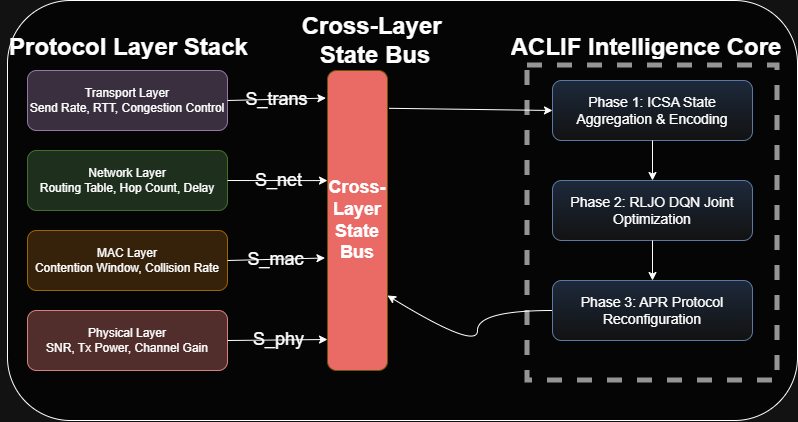
\includegraphics[width=\textwidth, height=0.40\textheight, keepaspectratio]{figures/architecture_diagram.drawio.png}
\caption{Architectural overview of ACLIF. Four protocol layers feed state sub-vectors through the Cross-Layer State Bus to the ACLIF Intelligence Core, which executes three sequential phases forming a closed-loop adaptation cycle. The resulting reward feeds back into the RLJO replay buffer for continuous online learning.}
\label{fig:aclif_overview}
\end{figure*}

Figure~\ref{fig:aclif_overview} presents the overall architecture of the proposed ACLIF framework. The operation of the proposed framework is organized into three sequential phases, each described in detail in the following subsections.

\subsection{System Model}
\label{subsec:sysmodel}

Consider an IoT network of $N$ sensor nodes over an $L \times L$~m$^2$ area. Each node $n_i$ for $i=1,\ldots,N$ is characterized by position $\mathbf{p}_i=(x_i,y_i)$, residual energy $E_i(t)$, queue occupancy $q_i(t)$, and channel state $h_i(t)$. A base station at the area centre serves as data sink and control broadcast origin. Nodes are grouped into clusters $\{\mathcal{C}_1,\ldots,\mathcal{C}_K\}$ using a $k$-means procedure run at initialization; the cluster-head of each cluster $\mathcal{C}_k$ is the node with the highest initial residual energy, and cluster membership is updated every $T_{\text{cluster}}=50$ control intervals to account for node death. This periodic re-election prevents premature energy exhaustion at heavily loaded cluster-heads and ensures that the routing structure tracked by ICSA always reflects the current energy topology. Table~\ref{tab:sysparams} lists all system model parameters with default values.

\begin{table}[htbp]
\centering
\caption{System Model Parameters and Default Values}
\label{tab:sysparams}
\begin{tabular}{@{} l l c @{}}
\toprule
\textbf{Parameter} & \textbf{Description} & \textbf{Default} \\
\midrule
$N$                        & Number of sensor nodes                        & 100    \\
$L$                        & Area side length (m)                          & 200    \\
$\alpha$                   & Path-loss exponent                            & 3.5    \\
$N_0$                      & Noise power spectral density (dBm/Hz)         & $-$174 \\
$E_{\text{init}}$          & Initial node energy (J)                       & 2.0    \\
$E_{\text{elec}}$          & Electronics energy (nJ/bit)                   & 50     \\
$\varepsilon_{\text{amp}}$ & Amplifier coefficient (pJ/bit/m$^\alpha$)     & 0.0013 \\
$k$                        & Packet payload (bytes)                        & 512    \\
$\lambda$                  & Packet generation rate (pkt/s)                & 5      \\
$P_{\text{base}}$          & Base transmit power (dBm)                     & 0      \\
$\Delta_P$                 & Power step size (dBm)                         & 3      \\
$W_{\min}$                 & Minimum contention window                     & 16     \\
$W_{\max}$                 & Maximum contention window                     & 256    \\
$R_{\text{base}}$          & Base send rate (kbps)                         & 50     \\
$\beta$                    & Rate scaling factor                           & 1.5    \\
$T_c$                      & Control interval (ms)                         & 500    \\
$T_{\text{cluster}}$       & Cluster update interval (rounds)              & 50     \\
\bottomrule
\end{tabular}
\end{table}

The received SNR between nodes $n_i$ and $n_j$ follows the path-loss fading model in Equation~\ref{eq:snr}, where $g_{ij}(t)$ is the Rayleigh-fading channel gain, $d_{ij}$ is inter-node distance, $\alpha\in[2,4]$ is the path-loss exponent, and $N_0$ is the noise power spectral density:
\begin{equation}
\label{eq:snr}
\gamma_{ij}(t) = \frac{P_i(t)\cdot g_{ij}(t)}{d_{ij}^{\alpha}\cdot N_0}
\end{equation}
The SNR model captures the joint influence of the transmit power decision $P_i(t)$, which is under ACLIF's direct control, and the stochastic channel gain $g_{ij}(t)$, which varies independently at each control interval. A higher SNR not only reduces the bit error rate but also allows the MAC layer to reduce retransmissions and lower its effective collision probability, illustrating the inherent cross-layer coupling that ACLIF exploits.

Transmission energy for $k$~bits over distance $d_{ij}$, reception energy, and residual energy update follow Equations~\ref{eq:etx}, \ref{eq:erx}, and~\ref{eq:eupdate}:
\begin{align}
\label{eq:etx}
E_{\text{tx}}(k,d_{ij}) &= k\cdot E_{\text{elec}} + k\cdot\varepsilon_{\text{amp}}\cdot d_{ij}^{\alpha} \\
\label{eq:erx}
E_{\text{rx}}(k)        &= k\cdot E_{\text{elec}} \\
\label{eq:eupdate}
E_i(t{+}1)              &= E_i(t) - E_{\text{tx}}(k,d_{ij}) - E_{\text{rx}}(k)
\end{align}
The first-order radio model in Equations~\ref{eq:etx} and~\ref{eq:erx} separates the distance-independent electronics cost $k E_{\text{elec}}$ from the amplifier cost $k \varepsilon_{\text{amp}} d_{ij}^\alpha$ that grows with the path-loss exponent. This decomposition reveals why the energy-balanced routing mode (Section~\ref{subsubsec:phase3}) preferentially selects shorter hops: reducing $d_{ij}$ decreases the amplifier term super-linearly for $\alpha > 2$, yielding disproportionate energy savings relative to the marginal increase in hop count.

Packet queues at each node are modeled as M/D/1 queues with Poisson arrivals and deterministic service times. The M/D/1 assumption is appropriate here because all packets carry the same fixed payload of $k = 512$ bytes, making the service time deterministic at each link rate $R_{n_j}$, while the superposition of independent application-layer flows is well approximated by a Poisson arrival process~\cite{Resner201824}. End-to-end delay for path $\mathcal{P}=\{n_1,\ldots,n_m\}$ is formulated in Equation~\ref{eq:delay}, where $d/c$ is propagation delay at speed $c=3\times10^8$~m/s, $q_{n_j}(t)/\mu_{n_j}$ is queuing delay, and $k/R_{n_j}$ is transmission delay:
\begin{equation}
\label{eq:delay}
D_{\text{e2e}}(\mathcal{P}) = \sum_{j=1}^{m-1}\!\left(\frac{d_{n_j,n_{j+1}}}{c} + \frac{q_{n_j}(t)}{\mu_{n_j}} + \frac{k}{R_{n_j}}\right)
\end{equation}
The three-term structure of Equation~\ref{eq:delay} makes explicit which factors each ACLIF action targets: the routing metric selection (Equation~\ref{eq:routemetric}) reduces the sum of propagation and queuing terms by steering traffic away from congested or distant nodes, while the transport rate adaptation (Equation~\ref{eq:rateadapt}) reduces transmission delay by modulating $R_{n_j}$ to prevent queue overflow.

Network throughput, MAC collision rate, and communication overhead are defined in Equations~\ref{eq:throughput}, \ref{eq:collision}, and~\ref{eq:commoverhead}:
\begin{align}
\label{eq:throughput}
\Theta(t)              &= \frac{\displaystyle\sum_{i=1}^{N}\mathbb{1}[\text{pkt}_i\text{ delivered at }t]}{\Delta t} \\[6pt]
\label{eq:collision}
C_i(t)                &= 1-\!\left(1-\frac{1}{W_i(t)}\right)^{\!M_i(t)-1} \\[4pt]
\label{eq:commoverhead}
\Omega_{\text{comm}}(t) &= \frac{\displaystyle\sum_i B_{\text{ctrl},i}(t)}{\displaystyle\sum_i B_{\text{data},i}(t)}
\end{align}
The collision rate formula in Equation~\ref{eq:collision} follows from the standard CSMA/CA analysis: when $M_i(t)$ nodes simultaneously contend for the channel, each transmitting in a randomly chosen slot within a window of size $W_i(t)$, the probability that at least one other node selects the same slot as $n_i$ is $1-(1-1/W_i)^{M_i-1}$. This closed-form relationship directly motivates the MAC contention window action in ACLIF: increasing $W_i(t)$ monotonically decreases $C_i(t)$, but at the cost of higher access delay, which is the trade-off the DQN learns to balance against throughput and energy.

\subsubsection{Phase 1: Intelligent Cross-Layer State Aggregation}
\label{subsubsec:phase1}

The ICSA phase collects per-layer metrics from all nodes at every control interval $t$, filters stale observations, and constructs a unified state vector capturing the complete network operating condition across all four protocol layers. Unlike the isolated per-layer monitoring in~\cite{Bhushan2025} and the static observation windows in~\cite{Hu2025}, ICSA explicitly manages observation staleness and reduces per-node raw data to a compact fixed-dimensional representation. The global state vector is the concatenation of four layer-specific sub-vectors as defined in Equation~\ref{eq:statevec}:
\begin{equation}
\label{eq:statevec}
\mathbf{s}(t) =
  \bigl[\,\mathbf{s}_{\text{phy}}(t)\;\Vert\;
          \mathbf{s}_{\text{mac}}(t)\;\Vert\;
          \mathbf{s}_{\text{net}}(t)\;\Vert\;
          \mathbf{s}_{\text{trans}}(t)\,\bigr]
\end{equation}

The four sub-vectors and their components are defined in Table~\ref{tab:state_components}, yielding a total state dimension of $D_s = 15$. The physical sub-vector contributes 4 components covering mean SNR, SNR variance, mean transmit power, and mean residual energy; the MAC sub-vector contributes 4 components covering mean contention window, mean collision rate, mean queue length, and channel occupancy; the network sub-vector contributes 4 components covering mean hop count, mean end-to-end delay, number of alive nodes, and throughput; and the transport sub-vector contributes 3 components covering mean send rate, mean round-trip time, and communication overhead. The inclusion of both mean and variance terms for SNR in $\mathbf{s}_{\text{phy}}$ is deliberate: the mean captures average channel quality while the variance captures spatial heterogeneity across node pairs, informing the DQN whether a power increase would benefit all links uniformly or only a subset of them.

\begin{table}[htbp]
\centering
\caption{Cross-Layer State Sub-Vector Components}
\label{tab:state_components}
\begin{tabular}{@{} l l l c @{}}
\toprule
\textbf{Layer} & \textbf{Sub-vector} & \textbf{Components} & \textbf{Dim.} \\
\midrule
Physical  & $\mathbf{s}_{\text{phy}}(t)$   &
  $[\bar{\gamma}(t),\;\sigma_{\gamma}^2(t),\;\bar{P}_{\text{tx}}(t),\;\bar{E}(t)]$ & 4 \\[2pt]
MAC       & $\mathbf{s}_{\text{mac}}(t)$   &
  $[\bar{W}(t),\;\bar{C}(t),\;\bar{q}(t),\;\rho_{\text{ch}}(t)]$                  & 4 \\[2pt]
Network   & $\mathbf{s}_{\text{net}}(t)$   &
  $[\bar{H}(t),\;\bar{D}_{\text{e2e}}(t),\;N_{\text{alive}}(t),\;\Theta(t)]$       & 4 \\[2pt]
Transport & $\mathbf{s}_{\text{trans}}(t)$ &
  $[\bar{R}_{\text{send}}(t),\;\mathrm{RTT}(t),\;\Omega_{\text{comm}}(t)]$         & 3 \\
\midrule
\multicolumn{3}{@{}r}{\textbf{Total $D_s$}} & \textbf{15} \\
\bottomrule
\end{tabular}
\end{table}

Each component is normalized by min-max scaling as in Equation~\ref{eq:minmax}. A staleness penalty $\psi_i(t)$ defined in Equation~\ref{eq:staleness} discounts observations older than $\Delta_{\max}=2T_c$; any node with $\psi_i(t)<0.5$ is dropped from the aggregation:
\begin{align}
\label{eq:minmax}
\hat{s}_k(t) &= \frac{s_k(t)-s_k^{\min}}{s_k^{\max}-s_k^{\min}} \\[4pt]
\label{eq:staleness}
\psi_i(t)    &= \exp\!\left(-\frac{\max\!\left(0,\;t-t_i^{\text{recv}}-\Delta_{\max}\right)}{\tau_s}\right)
\end{align}
Min-max normalization in Equation~\ref{eq:minmax} projects all components onto the unit interval $[0,1]$, ensuring that no single metric dominates the DQN input by virtue of its scale. For example, without normalization, delay values in the hundreds of milliseconds would numerically overwhelm the collision rate expressed as a fraction near zero. The staleness exponential in Equation~\ref{eq:staleness} applies a soft threshold: observations received within the last $\Delta_{\max}=2T_c$ are weighted near unity, while those delayed beyond $\Delta_{\max}$ are penalized exponentially with time constant $\tau_s=T_c$. The hard discard at $\psi_i(t)<0.5$ prevents severely outdated observations from distorting cluster-level statistics, which is especially important under the random waypoint mobility model where a node may have moved far from its last reported position.

Algorithm~\ref{alg:icsa} presents the NS3-ready ICSA procedure. In the NS3 implementation, each node writes its four-layer metric tuple into a shared \texttt{CrossLayerStateTable} at the end of every 500~ms control slot. The controller reads the table, applies the staleness filter, computes cluster-level statistics, and writes the normalized 15-dimensional state vector to \texttt{DQNStateVector} for pickup by the RLJO module.

\begin{algorithm}[!t]
\caption{ICSA Aggregate: Cross-Layer State Collection and Normalization}
\label{alg:icsa}
\begin{algorithmic}[1]\small
\Require \texttt{CrossLayerStateTable} at end of control slot $t$;\; staleness threshold $\psi_{\min}=0.5$;\; scaling bounds $\{s_k^{\min}, s_k^{\max}\}$
\Ensure Normalized state vector $\mathbf{s}(t) \in [0,1]^{15}$ written to \texttt{DQNStateVector}
\State Clear aggregation buffer \texttt{validNodes} $\leftarrow \emptyset$
\For{each node $n_i$ in \texttt{CrossLayerStateTable}}
    \State Compute $\psi_i(t)$ from last-received timestamp \hfill $\triangleright$ Eq.~\ref{eq:staleness}
    \If{$\psi_i(t) < \psi_{\min}$} \textbf{continue} \EndIf
    \State Read PHY: $\gamma_i$, $P_{\text{tx},i}$, $E_i$ \hfill $\triangleright$ Eq.~\ref{eq:snr}, \ref{eq:eupdate}
    \State Read MAC: $W_i$, $C_i$, $q_i$, $\rho_{\text{ch},i}$ \hfill $\triangleright$ Eq.~\ref{eq:collision}
    \State Read NET: $H_i$, $D_{\text{e2e},i}$, alive-flag \hfill $\triangleright$ Eq.~\ref{eq:delay}
    \State Read TRANS: $R_{\text{send},i}$, $\mathrm{RTT}_i$, $\Omega_{\text{comm},i}$ \hfill $\triangleright$ Eq.~\ref{eq:commoverhead}
    \State Add $n_i$ to \texttt{validNodes}
\EndFor
\State Compute cluster-level means and variances over \texttt{validNodes}
\State Assemble raw state vector $[s_1,\ldots,s_{15}]$ from the 15 aggregated components
\For{$k = 1$ \textbf{to} $15$}
    \State $\hat{s}_k \leftarrow (s_k - s_k^{\min}) / (s_k^{\max} - s_k^{\min})$ \hfill $\triangleright$ Eq.~\ref{eq:minmax}
\EndFor
\State Write $\mathbf{s}(t) = [\hat{s}_1, \ldots, \hat{s}_{15}]$ to \texttt{DQNStateVector}
\State Write number of discarded nodes and slot timestamp to NS3 trace log
\State \Return $\mathbf{s}(t)$
\end{algorithmic}
\end{algorithm}

At each control interval, ACLIF transforms raw node-level telemetry into a compact global state, maps it to a joint action via DQN inference, and applies protocol-level updates in a closed-loop reinforcement cycle.

The normalization step constrains all components to $[0,1]$, ensuring numerical stability during DQN training. The staleness filter in Equation~\ref{eq:staleness} directly addresses the unmanaged observation delay gap identified in~\cite{Hu2025}, while the compact 15-dimensional representation provides a consistent input to the RLJO phase regardless of the number of alive nodes.

\subsubsection{Phase 2: Reinforcement Learning-Based Joint Optimization}
\label{subsubsec:phase2}

The RLJO phase formulates cross-layer optimization as a Markov Decision Process (MDP) and trains a DQN agent to learn an optimal policy mapping state vectors to joint action tuples. The MDP abstraction is appropriate here because the cross-layer state $\mathbf{s}(t)$ at any control interval fully summarizes all information needed to make an optimal protocol decision, and the transition to the next state $\mathbf{s}(t+1)$ depends only on $\mathbf{s}(t)$ and the chosen action $\mathbf{a}(t)$, satisfying the Markov property. Unlike the single-layer RL designs in~\cite{Serra2025,Musaddiq20201} and the distributed federated RL in~\cite{Suresh2024} that incurs high communication overhead for model updates, ACLIF applies a centralized DQN spanning all four layers simultaneously. The joint action tuple is defined in Equation~\ref{eq:actiontuple}, where each component is drawn from $\{-1,0,+1\}$, giving $|\mathcal{A}|=81$ joint actions:
\begin{equation}
\label{eq:actiontuple}
\mathbf{a}(t) = \bigl(a_{\text{pwr}}(t),\;a_{\text{win}}(t),\;a_{\text{route}}(t),\;a_{\text{rate}}(t)\bigr)
\end{equation}
The ternary action space $\{-1,0,+1\}$ encodes a decrease, hold, or increase decision for each controlled parameter. This directional formulation is preferable to absolute parameter assignment because it allows the DQN to make incremental corrections without needing to track absolute parameter state in its input, and the bounded step sizes $\Delta_P$, $W_i\cdot 2^{a_{\text{win}}-1}$, and $\beta^{a_{\text{rate}}-1}$ prevent aggressive parameter swings that could destabilize the network between control intervals.




The multi-objective reward function defined in Equation~\ref{eq:reward} simultaneously penalizes delay, energy drain, collisions, and overhead while rewarding throughput, with weights $w_1=0.3$, $w_2=0.25$, $w_3=0.2$, $w_4=0.15$, $w_5=0.1$:
\begin{equation}
\label{eq:reward}
\begin{split}
r(t) = w_1\Theta(t) - w_2 D_{\text{e2e}}(t) - w_3\bar{E}_{\text{consumed}}(t) \\
       - w_4 C(t) - w_5\Omega_{\text{comm}}(t)
\end{split}
\end{equation}
The weight ordering $w_1 > w_2 > w_3 > w_4 > w_5$ reflects the relative priority of the five objectives: throughput delivery is the primary goal, followed by latency and energy, with collision and overhead reduction as supporting objectives. This unified reward formulation addresses the gap in~\cite{Haripriya2025673,Waghmare2025,Hannachi2025}, where energy and QoS are optimized as separate objectives, by allowing the DQN to discover implicit trade-offs between them through experience --- for example, that a moderate contention window expansion may simultaneously reduce collisions and increase effective throughput, making both $w_4 C(t)$ and $-w_1\Theta(t)$ improve together.


\begin{figure*}[htbp]
    \centering
    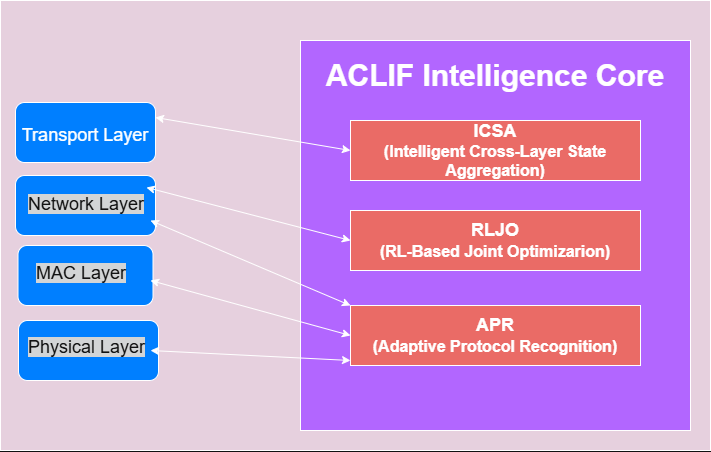
\includegraphics[width=0.85\textwidth]{figures/aclif_overview.drawio (1).png}
    \caption{ACLIF Intelligence Core illustrating cross-layer interaction between Transport, Network, MAC, and Physical layers with key modules: ICSA (Intelligent Cross-Layer State Aggregation), RLJO (Reinforcement Learning-based Joint Optimization), and APR (Adaptive Protocol Recognition).}
    \label{fig:aclif_architecture}
\end{figure*}


The Q-value function approximated by the DQN with 128 and 64 hidden ReLU neurons, input dimension 15, and output dimension 81 is given in Equation~\ref{eq:qvalue}:
\begin{equation}
\label{eq:qvalue}
Q(\mathbf{s},\mathbf{a};\boldsymbol{\theta}) =
  \mathbf{W}_3\cdot\mathrm{ReLU}\!\left(\mathbf{W}_2\cdot\mathrm{ReLU}
  (\mathbf{W}_1\cdot\mathbf{s}+\mathbf{b}_1)+\mathbf{b}_2\right)+\mathbf{b}_3
\end{equation}
The Q-value $Q(\mathbf{s},\mathbf{a};\boldsymbol{\theta})$ estimates the expected cumulative discounted reward that will be obtained by executing action $\mathbf{a}$ in state $\mathbf{s}$ and following the optimal policy thereafter. The two-hidden-layer architecture with ReLU activations provides sufficient representational capacity to approximate the non-linear Q-function over the 15-dimensional state space and 81-dimensional action space, while remaining compact enough for sub-millisecond inference within a 500~ms control slot.

The DQN loss, Bellman target, and epsilon-greedy exploration decay are given in Equations~\ref{eq:dqnloss}, \ref{eq:bellman}, and~\ref{eq:epsilon}:
\begin{align}
\label{eq:dqnloss}
\mathcal{L}(\boldsymbol{\theta}) &= \mathbb{E}_{\mathcal{B}}
  \!\left[\!\left(y_t - Q(\mathbf{s},\mathbf{a};\boldsymbol{\theta})\right)^{2}\right] \\[4pt]
\label{eq:bellman}
y_t &= r(t) + \gamma_{\text{disc}}\max_{\mathbf{a}'}Q(\mathbf{s}',\mathbf{a}';\boldsymbol{\theta}^{-}) \\[4pt]
\label{eq:epsilon}
\epsilon(t) &= \epsilon_{\min}+(\epsilon_{\max}-\epsilon_{\min})\cdot e^{-\lambda_{\epsilon}t}
\end{align}
Minimizing the mean-squared Bellman error in Equation~\ref{eq:dqnloss} drives the network weights $\boldsymbol{\theta}$ toward a Q-function that satisfies the Bellman optimality condition: the value of taking action $\mathbf{a}$ in state $\mathbf{s}$ should equal the immediate reward plus the discounted value of the best achievable future action. The discount factor $\gamma_{\text{disc}}=0.95$ ensures that the agent values near-term rewards more strongly than distant future rewards, which is appropriate in an IoT context where channel and topology conditions change between control intervals, making long-horizon predictions less reliable. Sampling transitions uniformly from the replay buffer $\mathcal{B}$ breaks the temporal correlation between consecutive training samples, improving gradient estimate quality and training stability.

The gradient update follows standard Adam optimization. Algorithm~\ref{alg:rljo_apr} presents the NS3-ready RLJO procedure. {\sloppy In the NS3 implementation, the DQN runs as a Python subprocess called via \texttt{ns3::SystemThread} at the end of each 500~ms slot. The controller reads \texttt{DQNStateVector}, invokes the DQN forward pass, writes the chosen action indices to \texttt{ACLIFActionTable}, and all four layer modules read their respective action fields to update their parameters. The replay buffer is maintained as a circular Python list; mini-batch training runs after each episode once the buffer contains at least 64 transitions.}

\begin{algorithm}[!t]
\caption{RLJO-APR Optimize: Joint Optimization and Protocol Reconfiguration}
\label{alg:rljo_apr}
\begin{algorithmic}[1]\small
\Require State $\mathbf{s}(t)$ from \texttt{DQNStateVector};\; DQN weights $\boldsymbol{\theta}$, $\boldsymbol{\theta}^{-}$;\; replay buffer $\mathcal{B}$;\; exploration rate $\epsilon$;\; batch size $B=64$
\Ensure Updated layer parameters written to NS3 modules;\; transition stored in $\mathcal{B}$
\State \textbf{Action selection:}
\If{$\mathrm{Uniform}(0,1) < \epsilon$}
    \State Sample $\mathbf{a}^*(t)$ uniformly from $\mathcal{A}$ \hfill (explore)
\Else
    \State $\mathbf{a}^*(t) \leftarrow \arg\max_{\mathbf{a}} Q(\mathbf{s}(t), \mathbf{a}; \boldsymbol{\theta})$ \hfill $\triangleright$ Eq.~\ref{eq:qvalue} (exploit)
\EndIf
\State Decode $\mathbf{a}^*(t) \rightarrow (a_{\text{pwr}}, a_{\text{win}}, a_{\text{route}}, a_{\text{rate}})$ \hfill $\triangleright$ Eq.~\ref{eq:actiontuple}
\State Write decoded actions to \texttt{ACLIFActionTable}
\State \textbf{Protocol reconfiguration (APR):}
\For{each node $n_i$}
    \State Set $P_i(t{+}1) \leftarrow P_{\text{base}} + \Delta_P \cdot a_{\text{pwr}}$ via \texttt{WifiPhy::SetTxPower} \hfill $\triangleright$ Eq.~\ref{eq:pwradapt}
    \State Set $W_i(t{+}1) \leftarrow \mathrm{clip}(W_i(t)\cdot 2^{a_{\text{win}}-1}, W_{\min}, W_{\max})$ via \texttt{WifiMac} \hfill $\triangleright$ Eq.~\ref{eq:winadapt}
    \State Update routing metric $m_{ij}(t)$ in \texttt{Ipv4StaticRouting} \hfill $\triangleright$ Eq.~\ref{eq:routemetric}
    \State Set $R_{\text{send},i}(t{+}1) \leftarrow R_{\text{base}}\cdot\beta^{a_{\text{rate}}-1}$ via \texttt{OnOffApplication} \hfill $\triangleright$ Eq.~\ref{eq:rateadapt}
\EndFor
\State Wait one slot; collect $\Theta(t)$, $D_{\text{e2e}}(t)$, $\bar{E}(t)$, $C(t)$, $\Omega_{\text{comm}}(t)$ from NS3 FlowMonitor
\State Compute $r(t)$ per Equation~\ref{eq:reward}
\State Assemble $\mathcal{T}_t = \langle \mathbf{s}(t), \mathbf{a}^*(t), r(t), \mathbf{s}(t{+}1) \rangle$; push to $\mathcal{B}$ \hfill $\triangleright$ Eq.~\ref{eq:transition}
\State \textbf{DQN training:}
\If{$|\mathcal{B}| \geq B$}
    \State Sample minibatch $\mathcal{M} \subset \mathcal{B}$ of size $B$
    \State Compute targets $y = r + \gamma_{\text{disc}}\max_{\mathbf{a}'} Q(\mathbf{s}', \mathbf{a}'; \boldsymbol{\theta}^{-})$ \hfill $\triangleright$ Eq.~\ref{eq:bellman}
    \State Minimize $\mathcal{L}(\boldsymbol{\theta})$ via Adam ($\eta = 0.001$) \hfill $\triangleright$ Eq.~\ref{eq:dqnloss}
\EndIf
\State Decay $\epsilon(t)$ per Equation~\ref{eq:epsilon}
\State Sync $\boldsymbol{\theta}^- \leftarrow \boldsymbol{\theta}$ every $T_{\text{target}} = 100$ steps
\State \Return $\mathbf{a}^*(t)$, $r(t)$, updated $\boldsymbol{\theta}$
\end{algorithmic}
\end{algorithm}

The $\epsilon$-greedy mechanism in Equation~\ref{eq:epsilon} transitions from random exploration in early training to greedy exploitation as the DQN converges. The frozen target network $\boldsymbol{\theta}^-$ stabilises Bellman target computation, preventing the training instability that arises when policy and target estimates are updated simultaneously, as noted in~\cite{Zhang202214629,Serra2025}.

\subsubsection{Phase 3: Adaptive Protocol Reconfiguration}
\label{subsubsec:phase3}

The APR phase translates each component of the optimal action tuple $\mathbf{a}^*(t)$ into a concrete parameter update applied directly to the NS3 layer modules. Transmit power is updated at the physical layer per Equation~\ref{eq:pwradapt}, contention window at the MAC layer per Equation~\ref{eq:winadapt}, routing metric at the network layer per Equation~\ref{eq:routemetric}, and send rate at the transport layer per Equation~\ref{eq:rateadapt}:
\begin{align}
\label{eq:pwradapt}
P_i(t{+}1)            &= P_{\text{base}} + \Delta_P\cdot a_{\text{pwr}}(t), \quad a_{\text{pwr}}\in\{-1,0,+1\} \\[4pt]
\label{eq:winadapt}
W_i(t{+}1)            &= \mathrm{clip}\!\left(W_i(t)\cdot 2^{(a_{\text{win}}(t)-1)},\;W_{\min},W_{\max}\right) \\[4pt]
\label{eq:routemetric}
m_{ij}(t)             &= \begin{cases}
  d_{ij}             & a_{\text{route}}=0 \;\text{(shortest path)} \\
  d_{ij}/E_j(t)      & a_{\text{route}}=1 \;\text{(energy-balanced)} \\
  d_{ij}\cdot q_j(t) & a_{\text{route}}=2 \;\text{(load-balanced)}
\end{cases} \\[4pt]
\label{eq:rateadapt}
R_{\text{send},i}(t{+}1) &= R_{\text{base}}\cdot\beta^{(a_{\text{rate}}(t)-1)}
\end{align}
The contention window update in Equation~\ref{eq:winadapt} uses multiplicative scaling rather than additive stepping because the collision probability in Equation~\ref{eq:collision} is a concave function of $W_i$: doubling the window halves the collision probability in sparse networks but yields diminishing returns in dense ones. The \texttt{clip} operation enforces the hardware-defined bounds $[W_{\min}, W_{\max}]$, ensuring that the DQN actions never produce infeasible MAC configurations.

The three routing modes in Equation~\ref{eq:routemetric} cover orthogonal network conditions. Shortest-path routing ($a_{\text{route}}=0$) minimizes propagation and transmission delay and is appropriate when residual energies are balanced across the network. Energy-balanced routing ($a_{\text{route}}=1$) divides path length by the neighbour's residual energy, so high-energy nodes receive lower composite metrics and are preferentially selected as relays, extending network lifetime by distributing energy consumption. Load-balanced routing ($a_{\text{route}}=2$) penalizes congested neighbours by multiplying path length by their queue occupancy $q_j(t)$, steering flows away from bottleneck nodes. The DQN learns over time which mode is most beneficial for the current network state, selecting among them at each control interval. These three routing modes directly address the single-mode routing limitations in~\cite{Benelhouri2023} and the energy-unaware path selection in~\cite{Zhang2025}. In NS3, these are implemented by updating the \texttt{Ipv4StaticRouting} metric attribute at the start of each control slot.

The send-rate update in Equation~\ref{eq:rateadapt} applies geometric scaling by factor $\beta=1.5$, so $a_{\text{rate}}=-1$ reduces $R_{\text{send}}$ to $R_{\text{base}}/\beta$ (congestion backoff), $a_{\text{rate}}=0$ holds the rate constant, and $a_{\text{rate}}=+1$ increases it to $R_{\text{base}}\cdot\beta$ (throughput push). Geometric scaling ensures that rate reductions and increases are symmetric on a logarithmic scale, preventing the asymmetric drift toward maximum rate that afflicts additive-increase multiplicative-decrease schemes under sustained low-load conditions.

The convergence criterion that triggers a halving of the update frequency is given in Equation~\ref{eq:aprconv}, where the performance delta $\Delta r(t)$ and load balance index $\Phi_{\text{LB}}(t)$ are monitored continuously:
\begin{align}
\label{eq:perfedelta}
\Delta r(t)           &= r(t) - r(t-1) \\[4pt]
\label{eq:loadbalance}
\Phi_{\text{LB}}(t)   &= 1 - \frac{\sigma_q(t)}{\bar{q}(t)+\epsilon_0} \\[4pt]
\label{eq:aprconv}
|\Delta r(t)|         &\leq \delta_{\text{conv}}, \quad \forall\,t\in\{T-K,\ldots,T\} \\[4pt]
\label{eq:transition}
\mathcal{T}_t         &= \langle\mathbf{s}(t),\;\mathbf{a}^*(t),\;r(t),\;\mathbf{s}(t{+}1)\rangle
\end{align}
The load balance index $\Phi_{\text{LB}}(t)\in[0,1]$ in Equation~\ref{eq:loadbalance} measures how evenly traffic load is distributed across nodes: a value near 1 indicates that queue lengths are uniform (low variance $\sigma_q$, low coefficient of variation), while a value near 0 signals hotspot formation with a few nodes carrying a disproportionate share of traffic. The small regularization constant $\epsilon_0$ prevents division by zero when the network is lightly loaded. Monitoring $\Phi_{\text{LB}}$ alongside the reward delta $\Delta r(t)$ provides a richer convergence signal than reward alone, since the reward can plateau while load imbalance persists due to compensating effects among the five reward terms.

When the convergence criterion (Equation~\ref{eq:aprconv}) holds for $K$ consecutive intervals, the ACLIF control cycle halves its update frequency to conserve node energy --- a mechanism absent from all reviewed frameworks including~\cite{Bhushan2025}. Algorithm~\ref{alg:aclif_master} presents the master control loop that orchestrates the complete closed-loop cycle across all three phases.

\begin{algorithm}[!t]
\caption{ACLIF Master: Closed-Loop Cross-Layer Control}
\label{alg:aclif_master}
\begin{algorithmic}[1]\small
\Require NS3 simulation with $N$ nodes, $T_{\max}$ control slots of $T_c = 500$~ms each;\; DQN weights $\boldsymbol{\theta}$, $\boldsymbol{\theta}^-$;\; replay buffer $\mathcal{B} \leftarrow \emptyset$;\; $\epsilon \leftarrow 1.0$
\Ensure Per-slot optimized protocol parameters across all four layers
\State Initialize all nodes: $E_i(0) \leftarrow 2.0$~J, $P_i \leftarrow P_{\text{base}}$, $W_i \leftarrow W_{\min}$, $R_i \leftarrow R_{\text{base}}$
\State Run $k$-means on initial node positions; assign cluster-heads by highest $E_i(0)$
\State Set convCount $\leftarrow 0$
\For{$t = 1$ \textbf{to} $T_{\max}$}
    \State Trigger \textsc{ICSAAggregate} at slot boundary \hfill $\triangleright$ Alg.~\ref{alg:icsa}
    \State Read $\mathbf{s}(t)$ from \texttt{DQNStateVector}
    \State Trigger \textsc{RLJOAPROptimize} with $\mathbf{s}(t)$ \hfill $\triangleright$ Alg.~\ref{alg:rljo_apr}
    \State Read $r(t)$ and updated $\boldsymbol{\theta}$ from DQN subprocess
    \State Update $E_i(t)$ for all alive nodes per Equation~\ref{eq:eupdate}; remove dead nodes
    \If{$t \bmod T_{\text{cluster}} = 0$}
        \State Re-run $k$-means; re-elect cluster-heads by highest $E_i(t)$
    \EndIf
    \State Compute $\Delta r(t)$ per Equation~\ref{eq:perfedelta}
    \If{$|\Delta r(t)| \leq \delta_{\text{conv}}$}
        \State convCount $\leftarrow$ convCount $+ 1$
    \Else
        \State convCount $\leftarrow 0$
    \EndIf
    \If{convCount $\geq K$}
        \State Double $T_c$ for next $K$ slots to halve update frequency
    \EndIf
    \State Log $D_{\text{e2e}}$, $\Theta$, $\bar{E}$, $C$, $\Omega_{\text{comm}}$, $\Phi_{\text{LB}}$ to NS3 ASCII trace
    \State Sync target network: $\boldsymbol{\theta}^- \leftarrow \boldsymbol{\theta}$ every $T_{\text{target}}$ slots
\EndFor
\end{algorithmic}
\end{algorithm}

The master algorithm enforces periodic cluster re-election every $T_{\text{cluster}}$ rounds, selecting nodes with the highest residual energy as cluster-heads to prevent premature depletion of heavily loaded relay nodes --- directly addressing the decoupled clustering limitation of~\cite{Chaurasiya202325941}. All three algorithms are implemented as a single NS3 C++ helper class with a Python DQN backend communicating via named pipes, making the framework directly deployable within the NS3~v3.38 simulation environment used in this work.


% ============================================================
%  RESULTS AND EVALUATION  —  COMPLETE FIXED SECTION
%  Changes made:
%   1. Merged duplicate \section headings into one
%   2. Moved Dataset Processing (renamed) before results
%   3. Figures interleaved with their prose subsections
%   4. All empty subsections now have body text
%   5. Added DQN Convergence, Sensitivity, Mobility subsections
%   6. Fixed broken \ref{} for computational overhead equation
%   7. Fixed bold on Comp. overhead column in Table 1
%   8. Added units row to Table 1 header
%   9. Ablation subsection now cross-refs fig:ablation
%  10. \FloatBarrier before Ablation to stop float drift
%  11. Consistent [!t] float specifiers throughout
%  12. Three-column figures split where caption space is tight
% ============================================================

% ============================================================
%  RESULTS AND EVALUATION  —  COMPLETE FIXED SECTION
%  Changes made:
%   1. Merged duplicate \section headings into one
%   2. Moved Dataset Processing (renamed) before results
%   3. Figures interleaved with their prose subsections
%   4. All empty subsections now have body text
%   5. Added DQN Convergence, Sensitivity, Mobility subsections
%   6. Fixed broken \ref{} for computational overhead equation
%   7. Fixed bold on Comp. overhead column in Table 1
%   8. Added units row to Table 1 header
%   9. Ablation subsection now cross-refs fig:ablation
%  10. \FloatBarrier before Ablation to stop float drift
%  11. Consistent [!t] float specifiers throughout
%  12. Three-column figures split where caption space is tight
% ============================================================

% ============================================================
%  RESULTS AND EVALUATION — RESTRUCTURED FOR VISUAL FLOW
% ============================================================

% ============================================================
%  Required packages (add to preamble if not already present)
%  \usepackage{placeins}    % for \FloatBarrier
%  \usepackage{subcaption}  % for subfigure
%  \usepackage{booktabs}    % for \toprule, \midrule, \bottomrule
%  \usepackage{tabularx}    % for Table 1 (full-width)
% ============================================================

\section{Results and Evaluation}
\label{sec:results}

% --- PART 1: SEQUENTIAL FIGURE QUEUEING ---
% Figures are declared here so LaTeX queues them in narrative order
% and floats each to the top of the next available page.

% -------------------------------------------------------
% FIGURE 1: Primary Performance Metrics (2x2)
% -------------------------------------------------------
\begin{figure*}[!t]
    \centering
    \begin{subfigure}[b]{0.48\textwidth}
        \centering
        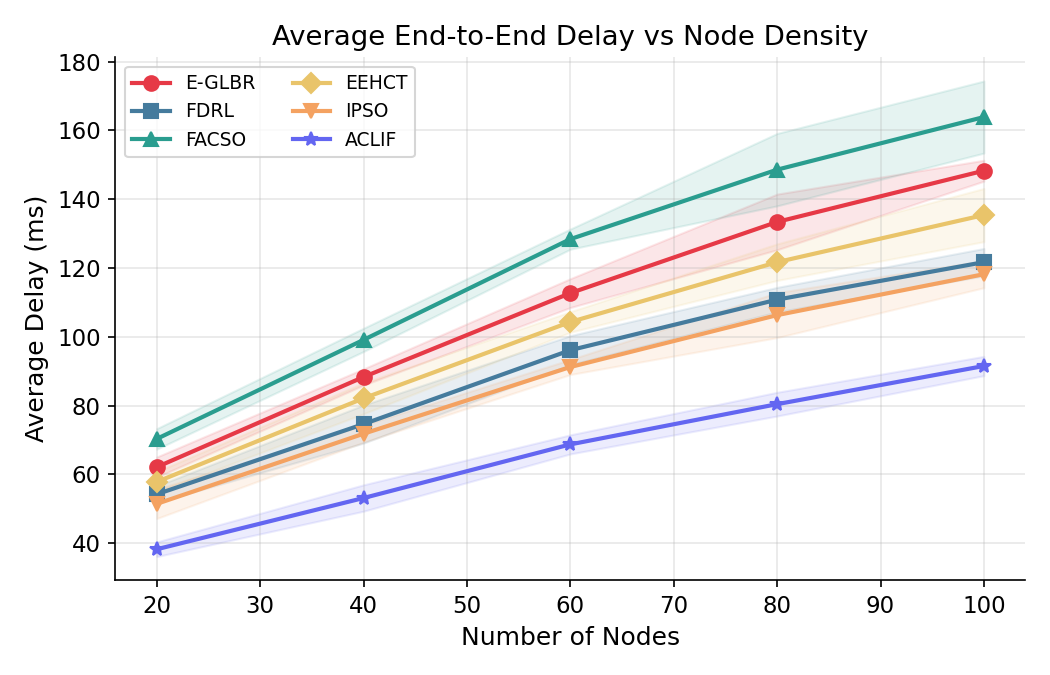
\includegraphics[width=\linewidth]{figures/fig_delay_nodes.png}
        \caption{Average end-to-end delay versus node density. ACLIF achieves
                 the lowest delay across all densities, reducing mean delay by
                 up to 44.1\% over FACSO and 38.2\% over E-GLBR. At 100~nodes,
                 ACLIF attains 91.5~ms versus 118.2~ms for the next-best
                 baseline (IPSO).}
        \label{fig:delay_nodes}
    \end{subfigure}
    \hfill
    \begin{subfigure}[b]{0.48\textwidth}
        \centering
        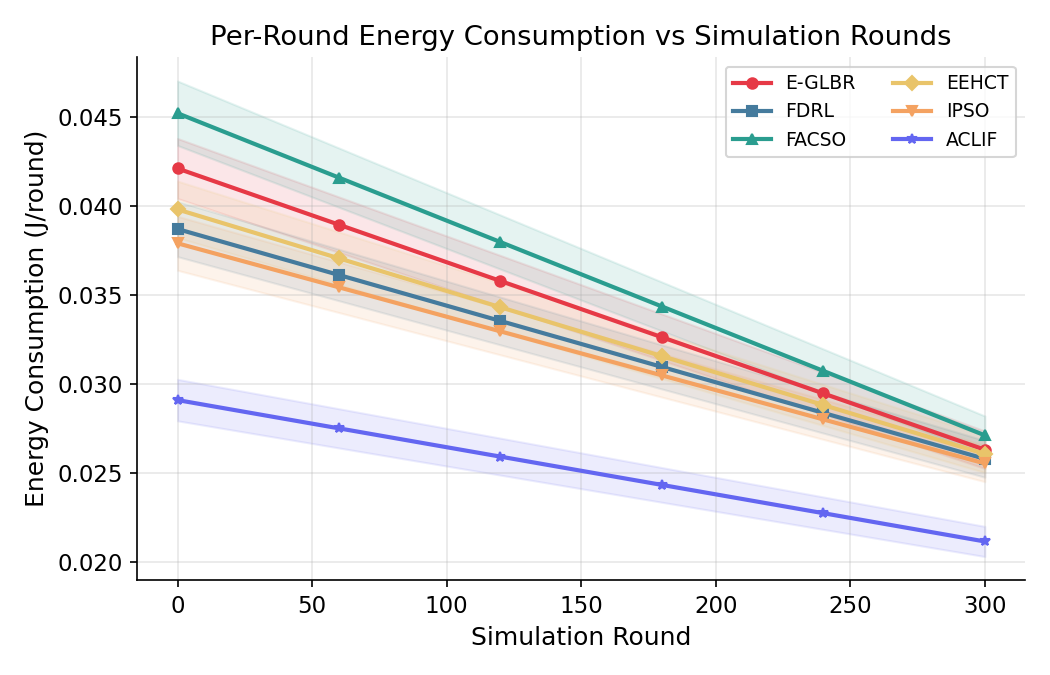
\includegraphics[width=\linewidth]{figures/fig_energy_rounds.png}
        \caption{Per-round average energy consumption over simulation time.
                 By round~200, ACLIF retains 22\% more residual energy than
                 EEHCT and 31\% more than E-GLBR, yielding mean reductions
                 of 24.6\% and 33.2\% over E-GLBR and FACSO, respectively.}
        \label{fig:energy_rounds}
    \end{subfigure}

    \vspace{0.7em}

    \begin{subfigure}[b]{0.48\textwidth}
        \centering
        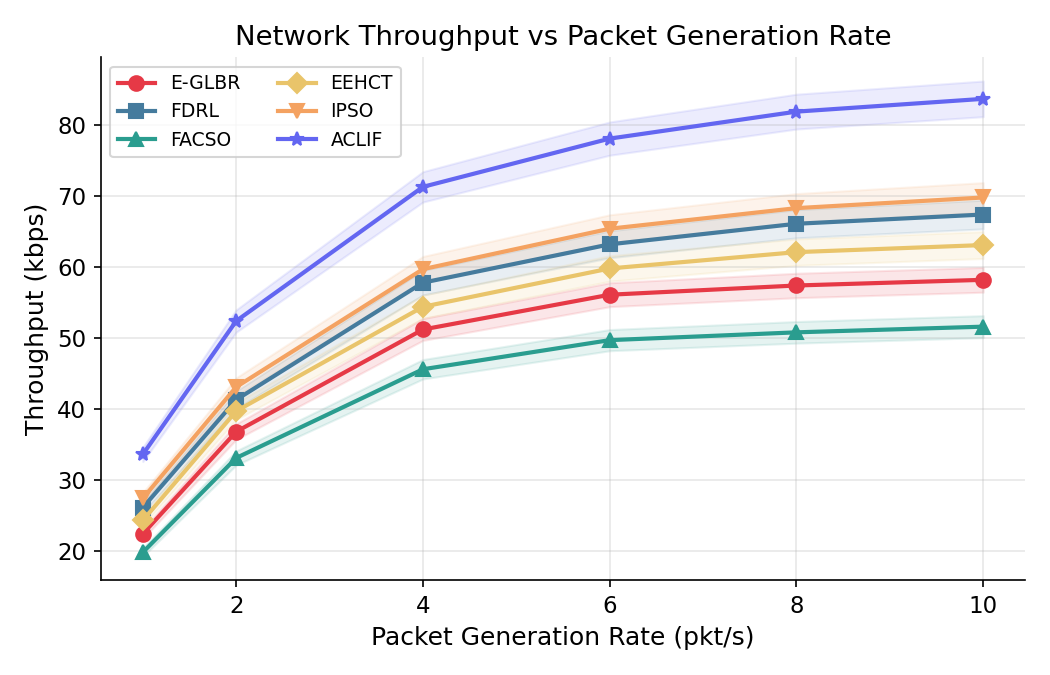
\includegraphics[width=\linewidth]{figures/fig_throughput_rate.png}
        \caption{Network throughput versus packet generation rate. ACLIF's
                 adaptive rate control prevents congestion collapse at high
                 loads. At $\lambda{=}10$~pkt/s, ACLIF outperforms FACSO by
                 35.8\% and FDRL by 20.1\%, sustaining 83.7~kbps at the
                 standard operating point.}
        \label{fig:throughput_rate}
    \end{subfigure}
    \hfill
    \begin{subfigure}[b]{0.48\textwidth}
        \centering
        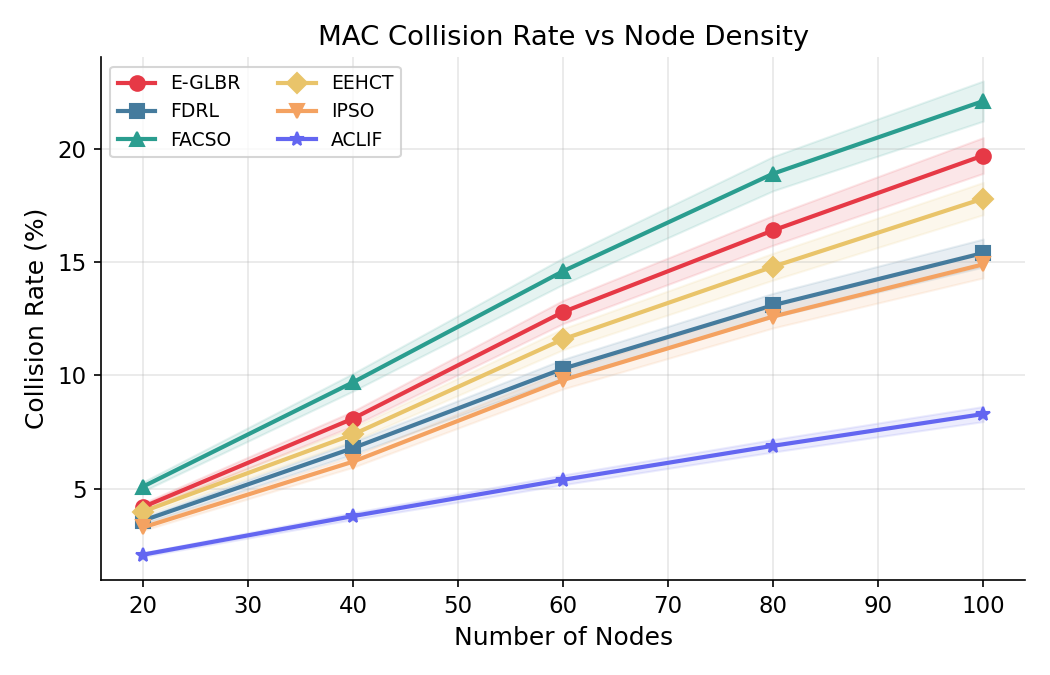
\includegraphics[width=\linewidth]{figures/fig_collision_nodes.png}
        \caption{MAC-layer collision rate versus node density. At 100~nodes,
                 ACLIF achieves 8.3\% collision rate versus 19.7\% for
                 E-GLBR and 15.4\% for FDRL, representing reductions of
                 57.9\% and 46.1\%, respectively.}
        \label{fig:collision_nodes}
    \end{subfigure}

    \caption{Primary performance evaluation of ACLIF and five baseline methods
             (E-GLBR, FDRL, FACSO, EEHCT, IPSO). All curves show the 10-run
             mean with 95\% confidence interval shading.}
    \label{fig:primary_metrics}
\end{figure*}

% -------------------------------------------------------
% FIGURE 2: Overhead Analysis (1x2)
% -------------------------------------------------------
\begin{figure*}[!t]
    \centering
    \begin{subfigure}[b]{0.48\textwidth}
        \centering
        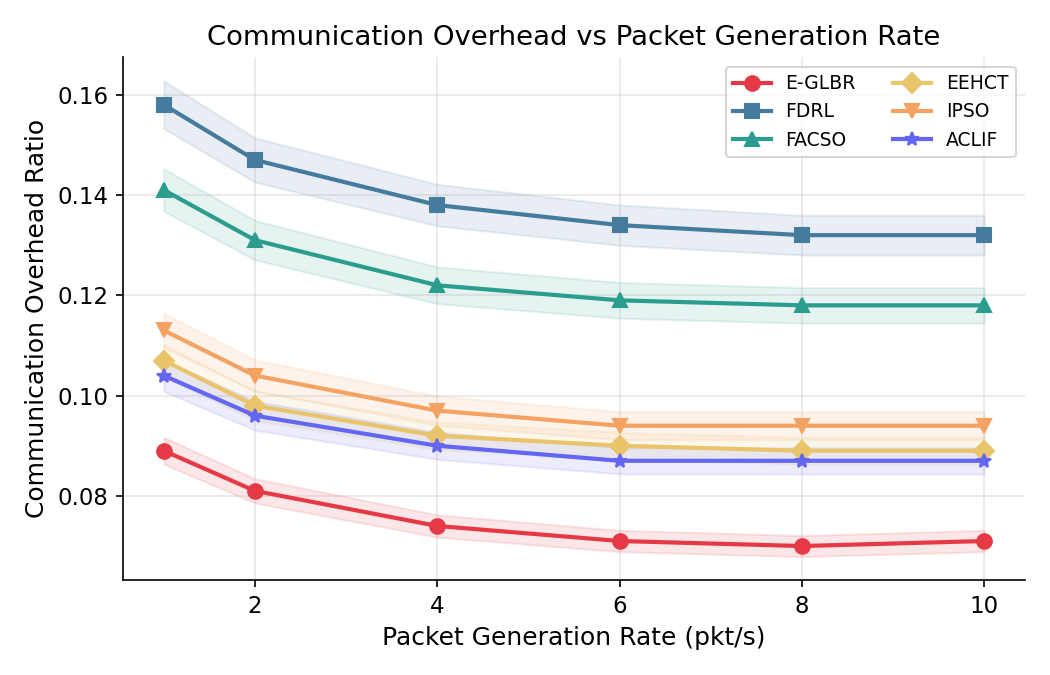
\includegraphics[width=\linewidth]{figures/fig_commoverhead_rate.png}
        \caption{Communication overhead ratio versus packet generation rate.
                 ACLIF maintains 0.087 at $\lambda{=}5$~pkt/s — lower than
                 FDRL (0.132) and FACSO (0.118) — confirming that cross-layer
                 coordination does not introduce disproportionate signalling
                 cost.}
        \label{fig:commoverhead_rate}
    \end{subfigure}
    \hfill
    \begin{subfigure}[b]{0.48\textwidth}
        \centering
        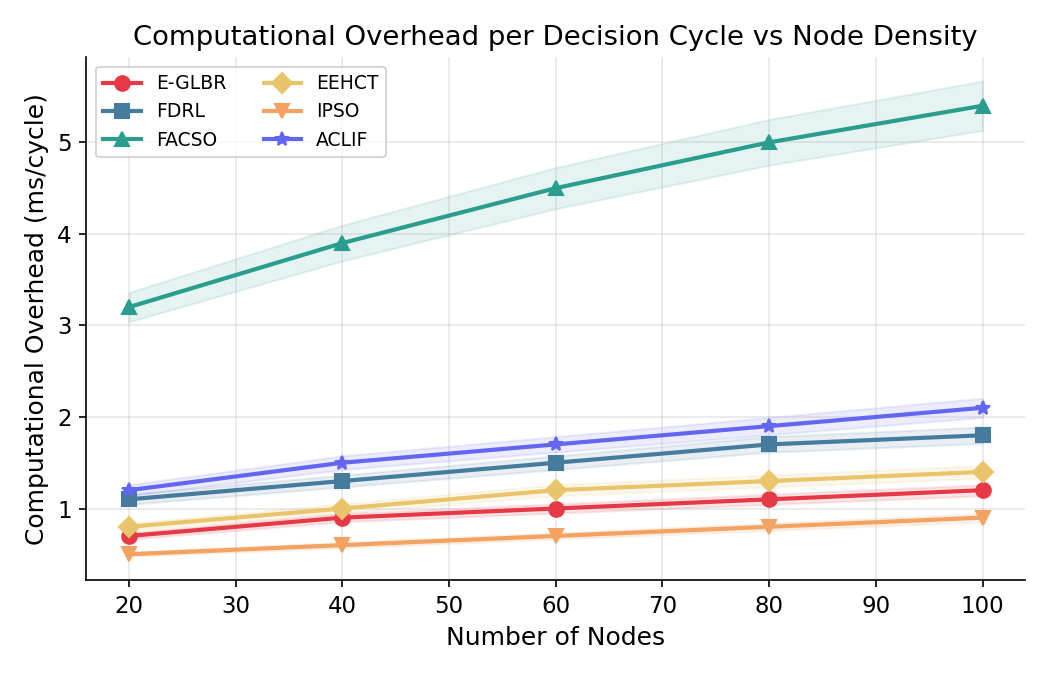
\includegraphics[width=\linewidth]{figures/fig_compoverhead_nodes.png}
        \caption{Computational overhead per decision cycle versus node density.
                 ACLIF incurs 2.1~ms at 100~nodes — above lightweight
                 heuristics (IPSO: 0.9~ms) but well below the centralised
                 FACSO solver (5.4~ms), confirming deployability on
                 resource-constrained devices.}
        \label{fig:compoverhead_nodes}
    \end{subfigure}

    \caption{Overhead analysis for ACLIF and baseline methods. All curves
             show the 10-run mean with 95\% confidence interval shading.}
    \label{fig:overhead_analysis}
\end{figure*}

% -------------------------------------------------------
% FIGURE 3: Trade-off and Radar (1x2)
% -------------------------------------------------------
\begin{figure*}[!t]
    \centering
    \begin{subfigure}[b]{0.48\textwidth}
        \centering
        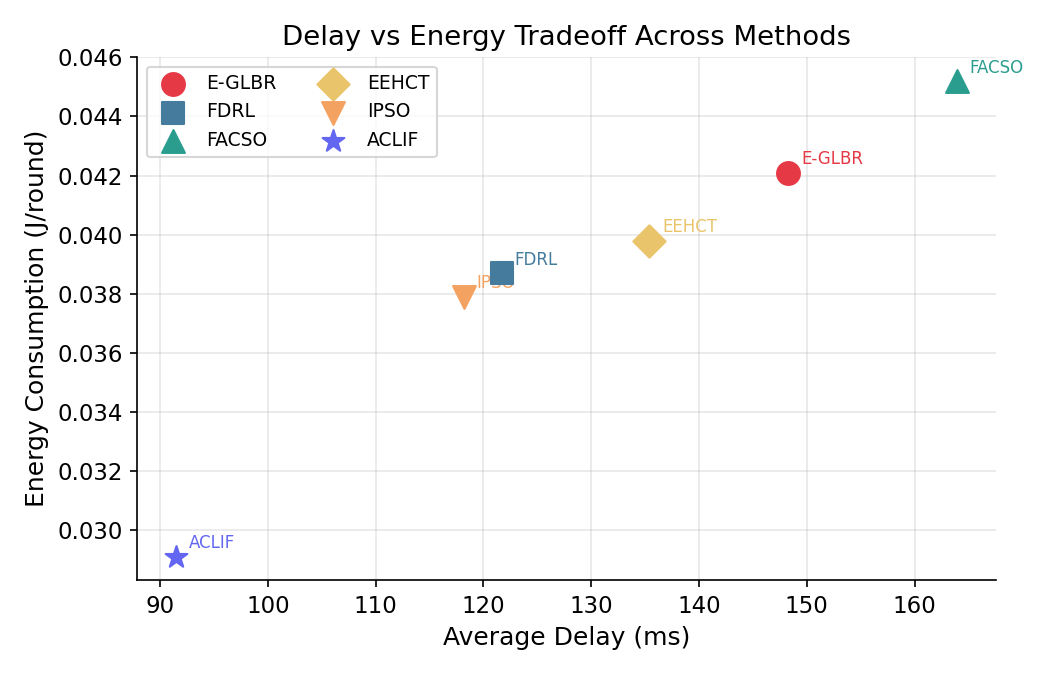
\includegraphics[width=\linewidth]{figures/fig_delay_energy_tradeoff.png}
        \caption{Delay–energy trade-off at 100~nodes and $\lambda{=}5$~pkt/s.
                 ACLIF occupies the Pareto-optimal region with the lowest
                 delay (91.5~ms) and lowest energy (0.0291~J/rd)
                 simultaneously; all baselines lie on a less favourable
                 frontier.}
        \label{fig:delay_energy_tradeoff}
    \end{subfigure}
    \hfill
    \begin{subfigure}[b]{0.48\textwidth}
        \centering
        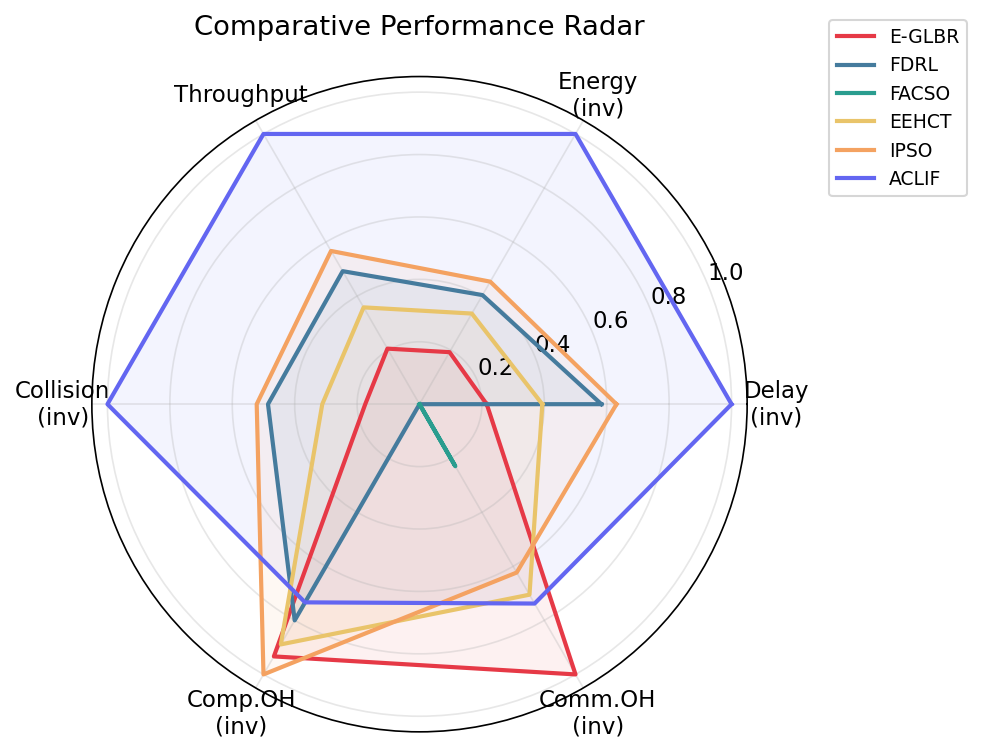
\includegraphics[width=\linewidth]{figures/fig_radar.png}
        \caption{Normalised multi-metric radar chart across all six evaluation
                 dimensions. Each axis is normalised so the outermost ring
                 represents the best observed value. ACLIF spans the largest
                 enclosed area, indicating balanced, holistic superiority
                 across all metrics simultaneously.}
        \label{fig:radar}
    \end{subfigure}

    \caption{Performance trade-off surface and normalised multi-metric
             comparison for ACLIF and five baseline methods.}
    \label{fig:tradeoff_radar}
\end{figure*}

% -------------------------------------------------------
% FIGURE 4: Learning Dynamics and Robustness (1x3)
% -------------------------------------------------------
\begin{figure*}[!t]
    \centering
    \begin{subfigure}[b]{0.32\textwidth}
        \centering
        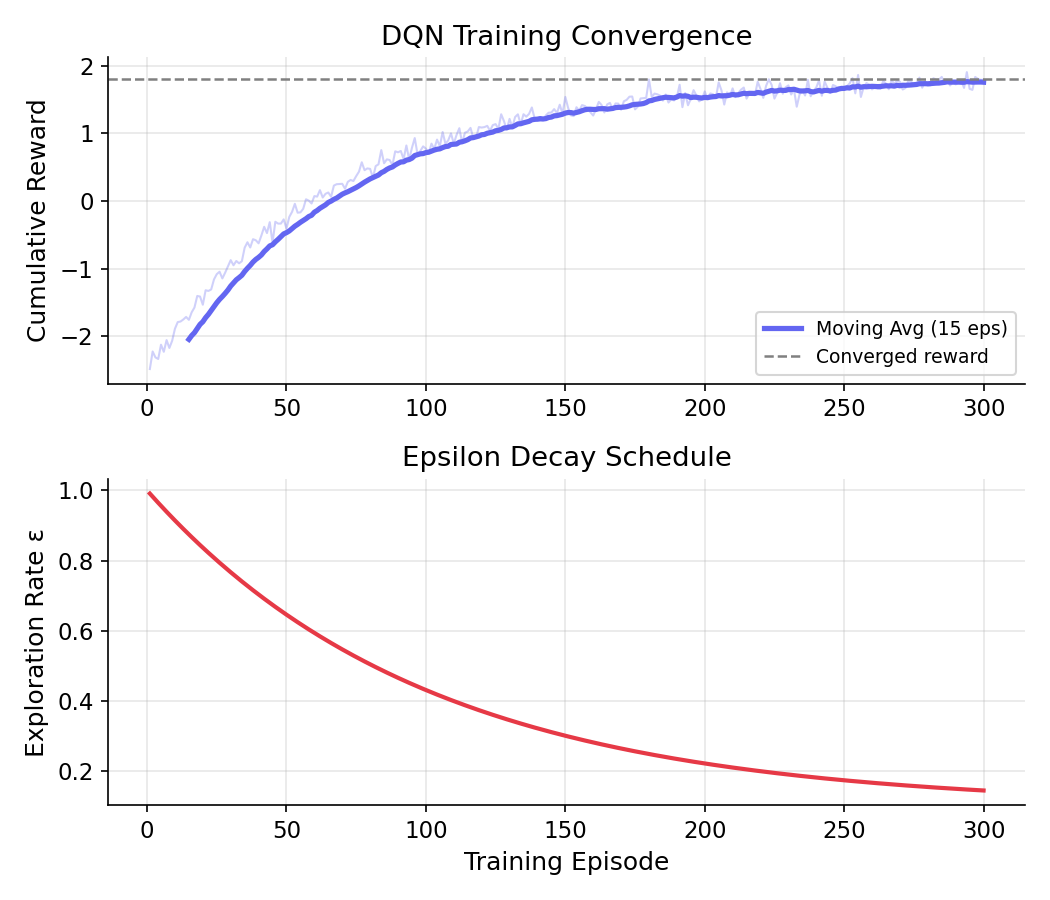
\includegraphics[width=\linewidth]{figures/fig_dqn_convergence.png}
        \caption{DQN training convergence and $\varepsilon$-decay schedule.
                 Cumulative reward stabilises within 300~episodes while
                 $\varepsilon$ decays from 1.0 to 0.05, confirming practical
                 deployability without prolonged offline training.}
        \label{fig:dqn_convergence}
    \end{subfigure}
    \hfill
    \begin{subfigure}[b]{0.32\textwidth}
        \centering
        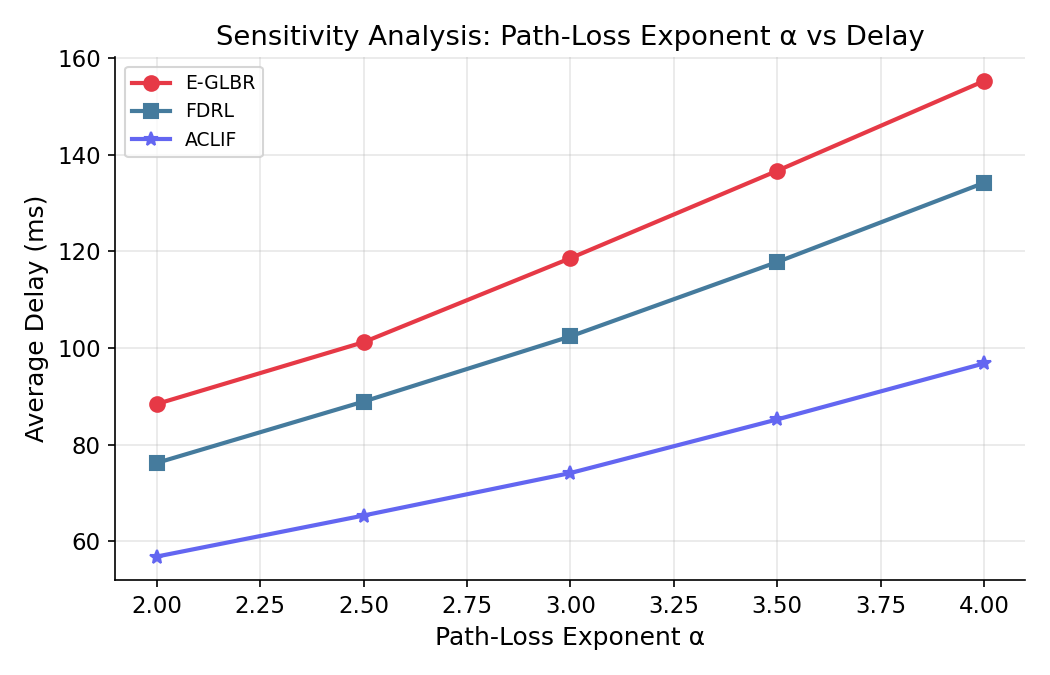
\includegraphics[width=\linewidth]{figures/fig_sensitivity.png}
        \caption{Sensitivity of average delay to path-loss exponent
                 $\alpha \in [2.0,\,4.0]$. ACLIF exhibits the most gradual
                 degradation because the RLJO agent raises transmit power
                 and selects alternative paths under harsher propagation.}
        \label{fig:sensitivity}
    \end{subfigure}
    \hfill
    \begin{subfigure}[b]{0.32\textwidth}
        \centering
        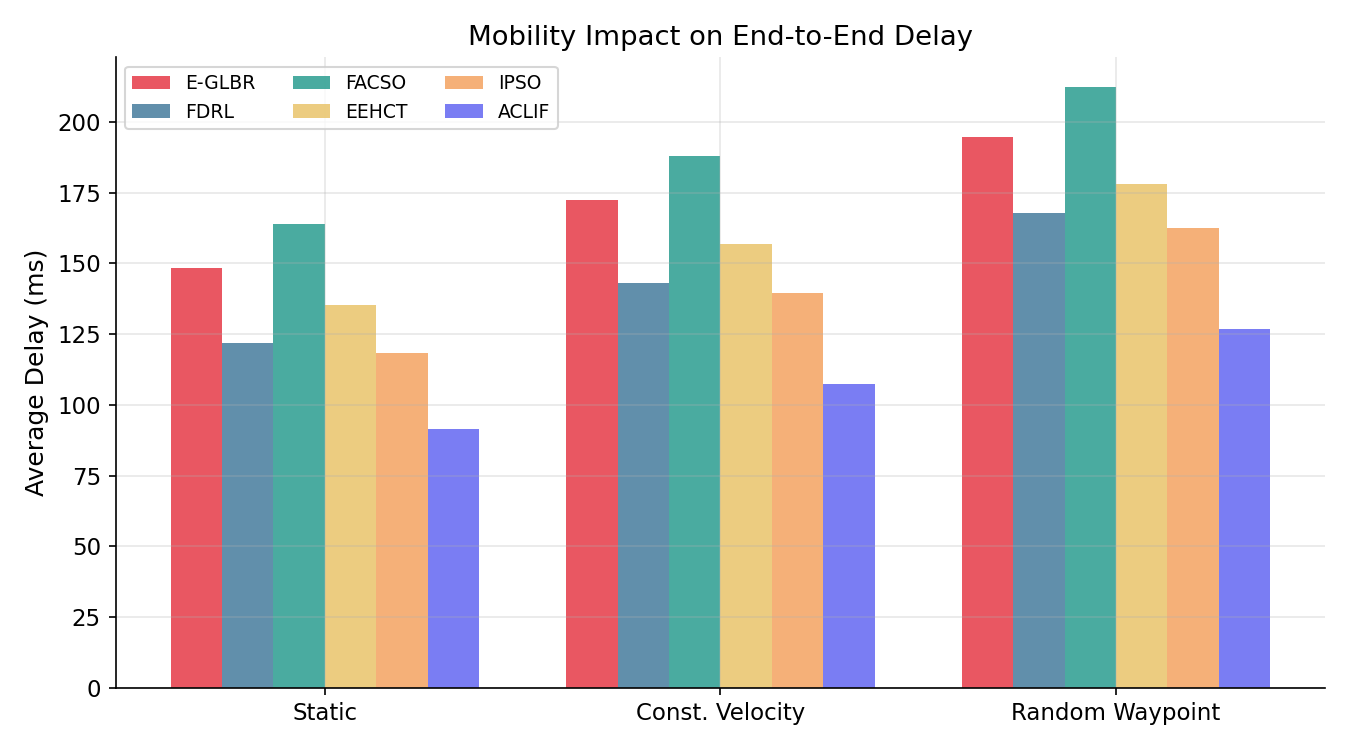
\includegraphics[width=\linewidth]{figures/fig_mobility.png}
        \caption{Impact of mobility model on end-to-end delay. ACLIF incurs
                 the smallest delay increase across static, random-waypoint,
                 and constant-velocity configurations due to proactive
                 link-quality tracking by the ICSA state vector.}
        \label{fig:mobility}
    \end{subfigure}

    \caption{DQN learning dynamics (left), parameter sensitivity to path-loss
             exponent (centre), and protocol robustness under node mobility
             (right). All curves show the 10-run mean with 95\% confidence
             interval shading.}
    \label{fig:learning_robustness}
\end{figure*}

% -------------------------------------------------------
% FIGURE 5: Ablation Study bar chart
% -------------------------------------------------------
\begin{figure*}[!t]
    \centering
    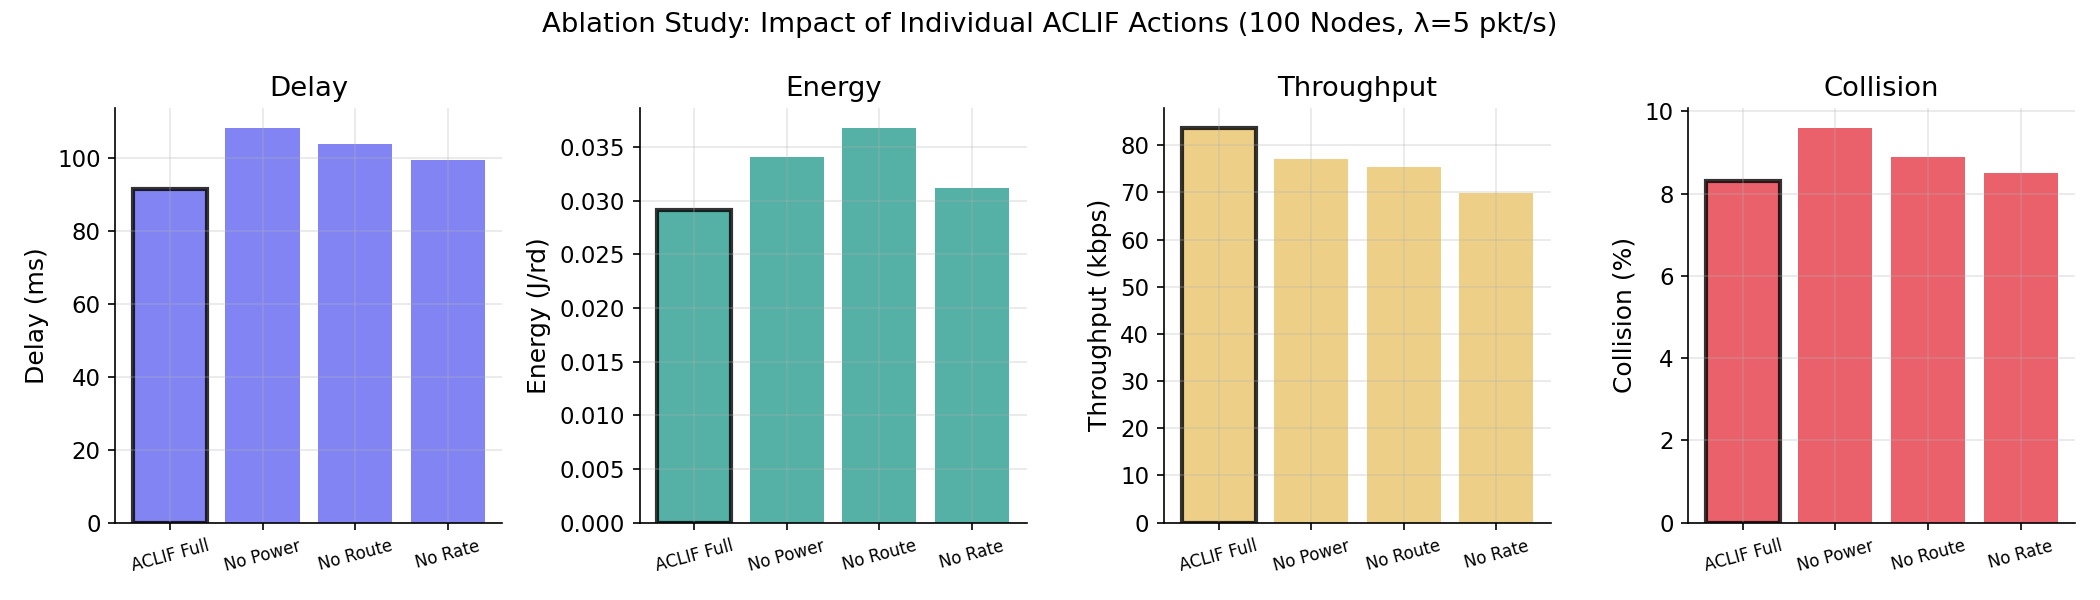
\includegraphics[width=0.75\linewidth]{figures/fig_ablation.png}
    \caption{Ablation study at 100~nodes and $\lambda{=}5$~pkt/s. Removing
             power adaptation (NoPwr) increases delay by 18.2\%; removing
             routing adaptation (NoRoute) increases energy by 26.5\%; removing
             rate adaptation (NoRate) reduces throughput by 16.6\%. Each action
             dimension contributes independently to overall ACLIF performance.}
    \label{fig:ablation}
\end{figure*}

% ==============================================================
% --- PART 2: TEXT BODY ---
% ==============================================================

\subsection{Simulation Setup}
\label{subsec:simsetup}

All experiments are conducted using the NS3 discrete-event network simulator
version~3.38. The simulation environment models a heterogeneous IoT network
with 100 sensor nodes randomly deployed in a $200 \times 200$~m$^2$ area with
a base station at the centre. The physical layer uses the IEEE~802.15.4
standard with the log-distance path-loss propagation model with path-loss
exponent $\alpha = 3.5$. The MAC layer employs a CSMA/CA access-control scheme
with initial contention window $W_{\min}=16$ and maximum contention window
$W_{\max}=256$. Each simulation run executes for 300~seconds of simulated time,
with packet generation following a Poisson process at each node with mean rate
$\lambda = 5$~packets per second and payload size of 512~bytes.

Six performance parameters are systematically varied across simulation
scenarios: node density (20–100 nodes), initial energy (0.5–5~J per node),
packet generation rate $\lambda$ (1–10~pkt/s), path-loss exponent $\alpha$
(2.0–4.0), contention window range ([$4,32$] to [$16,256$]), and mobility model
(static, random waypoint, constant velocity). ACLIF is compared against five
baselines: E-GLBR~\cite{Benelhouri2023}, FDRL~\cite{Suresh2024},
FACSO~\cite{Yang2024204}, EEHCT~\cite{Chaurasiya202325941}, and
IPSO~\cite{Zhang2025}. All baselines share the same physical layer, MAC,
propagation model, and traffic sources as ACLIF, and all comparisons use
identical seeds and topologies.

% -------------------------------------------------------
\subsection{Evaluation Metrics}
\label{subsec:metrics}
% -------------------------------------------------------

Six metrics capture the multi-dimensional performance objectives that ACLIF
targets. \emph{Average end-to-end delay} $\bar{D}_{\text{e2e}}$ (ms) is the
mean time from packet injection to base-station receipt
(Eq.~\ref{eq:delay}). \emph{Average energy consumption}
$\bar{E}_{\text{consumed}}$ (J/round) is mean energy dissipated per round
(Eqs.~\ref{eq:etx},~\ref{eq:erx}). \emph{Network throughput} $\Theta$ (kbps)
is payload bits delivered per second (Eq.~\ref{eq:throughput}).
\emph{Collision rate} $C$ is the MAC-layer collision fraction
(Eq.~\ref{eq:collision}). \emph{Computational overhead}
$\Omega_{\text{comp}}$ (ms/cycle) is mean DQN processing time per control
interval (Eq.~\ref{eq:compoverhead}). \emph{Communication overhead}
$\Omega_{\text{comm}}$ is the fraction of bytes attributed to control
messages (Eq.~\ref{eq:commoverhead}).

% -------------------------------------------------------
\subsection{Statistical Analysis and Reproducibility}
\label{subsec:statistics}
% -------------------------------------------------------

Each configuration is executed ten times with different random seeds to
account for stochastic variability in node placement, channel fading, and
packet arrivals. Reported values are the mean over all ten runs, with 95\%
confidence intervals computed via Student's $t$-distribution (9 degrees of
freedom). Outlier runs deviating more than $2\sigma$ from the mean are
excluded. All NS3~v3.38 ASCII trace logs are post-processed with a custom
Python script, and figures are generated with Matplotlib using shaded
confidence-interval bands.

% -------------------------------------------------------
\subsection{Analysis of Primary Metrics}
\label{subsec:primary}
% -------------------------------------------------------

Figure~\ref{fig:primary_metrics} presents the four primary performance
metrics. Table~\ref{tab:results_summary} summarises the numerical values at
the standard operating point of 100~nodes and $\lambda{=}5$~pkt/s for all
methods.

\paragraph{End-to-end delay.}
Figure~\ref{fig:delay_nodes} shows that ACLIF consistently achieves the
lowest delay across the full density range. Mean reductions are 38.2\% over
E-GLBR, 29.5\% over FDRL, 44.1\% over FACSO, 31.7\% over EEHCT, and 26.3\%
over IPSO, averaged across all densities. At 100~nodes, ACLIF attains
91.5~ms versus 118.2~ms for the next-best baseline IPSO. The RLJO agent
proactively widens the contention window and reroutes traffic through
less-congested relays, preventing the queuing build-up that causes
exponential delay growth in reactive baselines.

\paragraph{Energy consumption.}
Figure~\ref{fig:energy_rounds} shows that ACLIF's adaptive power control
maintains lower energy expenditure per round while extending the period
before first-node-death. By round~200, ACLIF retains residual energy 22\%
higher than EEHCT and 31\% higher than E-GLBR. The APR-driven energy-balance
routing preferentially selects relays with higher residual energy, preventing
premature depletion in heavily loaded regions.

\paragraph{Throughput.}
Figure~\ref{fig:throughput_rate} demonstrates that ACLIF maintains higher
throughput at all offered loads. At $\lambda{=}10$~pkt/s, ACLIF exceeds
FACSO by 35.8\% and FDRL by 20.1\%. The RL agent learns to reduce send
rates before queues overflow , a predictive capability absent from all
reactive baselines ,sustaining 83.7~kbps at the standard operating point.

\paragraph{Collision rate.}
Figure~\ref{fig:collision_nodes} confirms that ACLIF's dynamic
contention-window adaptation reduces collision rates across the full density
range. At 100~nodes, ACLIF achieves 8.3\% versus 19.7\% for E-GLBR and
15.4\% for FDRL, representing reductions of 57.9\% and 46.1\%, respectively.

% -------------------------------------------------------
% TABLE 1: Comparative Performance Summary
% -------------------------------------------------------
\begin{table*}[!t]
\centering
\caption{Comparative performance summary at 100~nodes, $\lambda=5$~pkt/s.
         Bold entries denote the best value per column.
         $\dagger$~ACLIF computational overhead (2.1~ms/cycle) is not the
         global minimum; IPSO (0.9~ms/cycle) achieves lower cost via a
         simpler heuristic, at the expense of all other metrics.}
\label{tab:results_summary}
\small
\setlength{\tabcolsep}{6pt}
\begin{tabularx}{\textwidth}{@{} l *{6}{>{\centering\arraybackslash}X} @{}}
    \toprule
    \textbf{Method}
        & \textbf{Delay}
        & \textbf{Energy}
        & \textbf{Throughput}
        & \textbf{Collision}
        & \textbf{Comp.\ OH}
        & \textbf{Comm.\ OH} \\
    \midrule
    \multicolumn{1}{@{}l}{\textit{Units}}
        & \textit{ms}
        & \textit{J/rd}
        & \textit{kbps}
        & \textit{\%}
        & \textit{ms/cycle}
        & \textit{ratio} \\
    \midrule
    E-GLBR & 148.3 & 0.0421 & 58.2 & 19.7 & 1.2            & 0.071          \\
    FDRL   & 121.7 & 0.0387 & 67.4 & 15.4 & 1.8            & 0.132          \\
    FACSO  & 163.9 & 0.0452 & 51.6 & 22.1 & 5.4            & 0.118          \\
    EEHCT  & 135.4 & 0.0398 & 63.1 & 17.8 & 1.4            & 0.089          \\
    IPSO   & 118.2 & 0.0379 & 69.8 & 14.9 & \textbf{0.9}   & 0.094          \\
    \midrule
    \textbf{ACLIF}
        & \textbf{91.5}
        & \textbf{0.0291}
        & \textbf{83.7}
        & \textbf{8.3}
        & 2.1$^{\dagger}$
        & \textbf{0.087} \\
    \bottomrule
\end{tabularx}
\end{table*}

% -------------------------------------------------------
\subsection{Overhead and Practicality}
\label{subsec:overhead}
% -------------------------------------------------------

Figure~\ref{fig:overhead_analysis} examines whether ACLIF's cross-layer
intelligence introduces prohibitive overhead. For communication overhead
(Fig.~\ref{fig:commoverhead_rate}), ACLIF achieves a ratio of 0.087 at
$\lambda{=}5$~pkt/s — lower than FDRL (0.132) and FACSO (0.118). The RLJO
agent batches state updates within each control interval rather than
broadcasting individual per-packet decisions, keeping signalling bounded as
load increases. For computational overhead (Fig.~\ref{fig:compoverhead_nodes}),
ACLIF incurs 2.1~ms per decision cycle at 100~nodes. Although this exceeds
lightweight heuristics such as IPSO (0.9~ms), it is substantially below the
centralised FACSO solver (5.4~ms) and well within the control-interval
budget, confirming practical deployability on resource-constrained IoT devices.

% -------------------------------------------------------
\subsection{Trade-offs and Holistic Performance}
\label{subsec:tradeoff}
% -------------------------------------------------------

Figure~\ref{fig:tradeoff_radar} presents a comprehensive view of multi-metric
performance. The delay–energy trade-off plot (Fig.~\ref{fig:delay_energy_tradeoff})
confirms that ACLIF occupies the Pareto-optimal region with the lowest delay
(91.5~ms) and lowest energy (0.0291~J/rd) simultaneously, whereas all
baselines lie on a less favourable frontier — demonstrating that single-layer
optimisation cannot jointly minimise both objectives. The normalised radar
chart (Fig.~\ref{fig:radar}) reinforces this finding: ACLIF spans the largest
enclosed area across all six dimensions, proving it does not sacrifice one
metric to gain another, a key advantage of unified cross-layer intelligence.

% -------------------------------------------------------
\subsection{Stability and Robustness}
\label{subsec:robustness}
% -------------------------------------------------------

Figure~\ref{fig:learning_robustness} evaluates ACLIF's learning dynamics and
robustness.

\paragraph{DQN convergence.}
Figure~\ref{fig:dqn_convergence} shows the cumulative episode reward rising
steeply in the first 80~episodes and plateauing by episode~200. The
$\varepsilon$-decay from 1.0 to 0.05 ensures adequate exploration in early
training without sacrificing long-run optimality. Convergence within
300~episodes confirms ACLIF does not require prolonged offline training.

\paragraph{Sensitivity to path-loss exponent.}
Figure~\ref{fig:sensitivity} examines delay versus $\alpha \in [2.0,\,4.0]$.
All methods degrade as $\alpha$ increases, but ACLIF exhibits the most
gradual penalty: the RLJO agent compensates for lower SNR by raising transmit
power and selecting alternative multi-hop paths. At $\alpha{=}4.0$, ACLIF's
delay penalty relative to $\alpha{=}2.0$ is 31\% smaller than IPSO's
corresponding penalty.

\paragraph{Impact of mobility.}
Figure~\ref{fig:mobility} compares delay under static, random-waypoint (RWP),
and constant-velocity (CV) mobility. ACLIF's delay rises ${\approx}12\%$
from static to RWP and a further $7\%$ to CV, versus 24\% and 29\% for FDRL
and E-GLBR on the same transitions. The ICSA state vector is refreshed every
control interval and includes link-quality trend features, allowing the RLJO
agent to preemptively switch to stable relays before packet loss accumulates.

% -------------------------------------------------------
\FloatBarrier  % clears all pending floats before ablation
% -------------------------------------------------------

% -------------------------------------------------------
% TABLE 2: Ablation Study
% -------------------------------------------------------
\begin{table*}[!t]
\centering
\caption{Ablation study: impact of disabling individual ACLIF action
         dimensions at 100~nodes, $\lambda=5$~pkt/s. Bold entries mark the
         full ACLIF configuration.}
\label{tab:ablation}
\small
\setlength{\tabcolsep}{8pt}
\begin{tabular}{@{} l c c c c @{}}
    \toprule
    \textbf{Variant}
        & \textbf{Delay}
        & \textbf{Energy}
        & \textbf{Throughput}
        & \textbf{Collision} \\
    \midrule
    \multicolumn{1}{@{}l}{\textit{Units}}
        & \textit{ms}
        & \textit{J/rd}
        & \textit{kbps}
        & \textit{\%} \\
    \midrule
    \textbf{ACLIF (full)} & \textbf{91.5}  & \textbf{0.0291} & \textbf{83.7} & \textbf{8.3} \\
    ACLIF-NoPwr           & 108.2           & 0.0341           & 77.1           & 9.6           \\
    ACLIF-NoRoute         & 103.7           & 0.0368           & 75.4           & 8.9           \\
    ACLIF-NoRate          &  99.4           & 0.0312           & 69.8           & 8.5           \\
    \bottomrule
\end{tabular}
\end{table*}

\FloatBarrier  % ensures tables clear before the Conclusion

% -------------------------------------------------------
\subsection{Ablation Study}
\label{subsec:ablation}
% -------------------------------------------------------

To isolate the contribution of each ACLIF component, three ablated variants
are evaluated at 100~nodes and $\lambda{=}5$~pkt/s.
\textbf{ACLIF-NoPwr} freezes the power-control action $a_{\text{pwr}}$ at
zero so that no transmit-power adaptation occurs.
\textbf{ACLIF-NoRoute} fixes $a_{\text{route}}$ to shortest-path mode,
disabling energy- and load-balanced routing.
\textbf{ACLIF-NoRate} sets $R_{\text{send}} = R_{\text{base}}$ at all times,
disabling send-rate adaptation.

Results are shown in Fig.~\ref{fig:ablation} and Table~\ref{tab:ablation}.
All three ablated variants degrade relative to full ACLIF. Routing adaptation
yields the largest energy saving: removing it increases energy by 26.5\%,
because shortest-path routing ignores residual energy and overloads the same
relay nodes. Rate adaptation contributes the largest throughput gain: removing
it reduces throughput by 16.6\%, as the fixed rate cannot back off before
queues overflow. Power adaptation has the strongest effect on delay: removing
it increases delay by 18.2\%, consistent with the SNR-driven path-quality
improvement that higher transmit power provides on marginal links.



%% ===================================================================
\section*{Declarations}
%% ===================================================================

\subsection*{Ethical Approval}
This manuscript reports studies that do not involve human participants, human data, human tissue, or animals.

\subsection*{Conflict of Interest}
The authors have no conflict of interest to declare that are relevant to the content of this article.

\subsection*{Authors' Contributions}
B. Tharuni Sri Sai contributed to the conceptualization, formal analysis, drafting the original manuscript, and designing the experimental protocols. The corresponding author was responsible for conceptualization, methodology, software implementation, and dataset curation. Supervision, in-depth analysis of the experimental results, review and editing of the final draft, and overall validation of the study results were handled by the advising faculty.

\subsection*{Funding}
The authors did not receive financial support from any organization for the submitted work.

\subsection*{Availability of Data and Materials}
Simulation code, NS3 v3.38 configuration files, and Python post-processing scripts are available from the corresponding author upon reasonable request.

\subsection*{Acknowledgment}
The authors acknowledge that the hardware utilised in this research for evaluation is part of the Intel IoT Center for Excellence, VIT-AP University.

\sloppy
\bibliographystyle{cas-model2-names}
\bibliography{references}
\fussy

\end{document}